
%%%%%%%%%%%%%%%%%%%%%%% file typeinst.tex %%%%%%%%%%%%%%%%%%%%%%%%%
%
% This is the LaTeX source for the instructions to authors using
% the LaTeX document class 'llncs.cls' for contributions to
% the Lecture Notes in Computer Sciences series.
% http://www.springer.com/lncs       Springer Heidelberg 2006/05/04
%
% It may be used as a template for your own input - copy it
% to a new file with a new name and use it as the basis
% for your article.
%
% NB: the document class 'llncs' has its own and detailed documentation, see
% ftp://ftp.springer.de/data/pubftp/pub/tex/latex/llncs/latex2e/llncsdoc.pdf
%
%%%%%%%%%%%%%%%%%%%%%%%%%%%%%%%%%%%%%%%%%%%%%%%%%%%%%%%%%%%%%%%%%%%


\documentclass[runningheads,a4paper]{llncs}
\usepackage{booktabs}
\usepackage{multirow}
\usepackage{amssymb}
\setcounter{tocdepth}{3}
\usepackage{graphicx}
\usepackage{makecell}
\usepackage{todonotes}

\usepackage{url}
\urldef{\mailsa}\path|{alfred.hofmann, ursula.barth, ingrid.haas, frank.holzwarth,|
\urldef{\mailsb}\path|anna.kramer, leonie.kunz, christine.reiss, nicole.sator,|
\urldef{\mailsc}\path|erika.siebert-cole, peter.strasser, lncs}@springer.com|    
\newcommand{\keywords}[1]{\par\addvspace\baselineskip
\noindent\keywordname\enspace\ignorespaces#1}

%\usepackage[table]{xcolor}

%\newcommand{\todo}[1]{\textcolor{red}{#1}}
\newcommand{\mytodo}[1]{\textcolor{red}{#1}}

\begin{document}

\mainmatter  % start of an individual contribution

\title{Understanding Document Understandability Through Correlation Analysis}
%\titlerunning{Running Title}

% a short form should be given in case it is too long for the running head
%\titlerunning{Lecture Notes in Computer Science: Authors' Instructions}

% the name(s) of the author(s) follow(s) next
%
% NB: Chinese authors should write their first names(s) in front of
% their surnames. This ensures that the names appear correctly in
% the running heads and the author index.
%
\author{Anonymous}
%
%\authorrunning{Lecture Notes in Computer Science: Authors' Instructions}
% (feature abused for this document to repeat the title also on left hand pages)

% the affiliations are given next; don't give your e-mail address
% unless you accept that it will be published
%\institute{Springer-Verlag, Computer Science Editorial,\\
%Tiergartenstr. 17, 69121 Heidelberg, Germany\\
%\mailsa\\
%\mailsb\\
%\mailsc\\
%\url{http://www.springer.com/lncs}}

%
% NB: a more complex sample for affiliations and the mapping to the
% corresponding authors can be found in the file "llncs.dem"
% (search for the string "\mainmatter" where a contribution starts).
% "llncs.dem" accompanies the document class "llncs.cls".
%

%\toctitle{Lecture Notes in Computer Science}
%\tocauthor{Authors' Instructions}
\maketitle


\section{Introduction}
\label{chp:understanding_understandability}

Recently, a number of works rely on the output of readability formulas to deem if a Web page is easy or hard to understand (e.g., \cite{graber99readability,fitzsimmons2010readability,wiener2013readability,patel13readability,atcherson14readability,meillier17readability}).
However, as discussed in Chapter~\ref{chp:preprocessing}, preprocessing steps are crucial for the interpretation of readability formula results. When applying them to assess the understandability of Web   document, the same readability formula may yield results that vary from \textit{suitable even for kids} to \textit{understandable only if you are an experts} with only minor modifications in the preprocessing steps.
In this chapter, we investigate if any of these two interpretations is correct analysing the correlations of various understandability estimators and human assessments.
For that, we take advantage of the understandability assessments made in recent CLEF eHealth campaigns (\cite{clef15,clef16}).

During the CLEF eHealth 2015 and 2016 campaigns \cite{clef15,clef16}, in addition to topical relevance, medical students and professional serving as assessors were instructed to assess how easy to understand and how much they would trust the information contained in each assessed document. The assessment tool used in these campaigns is shown in Figure~\ref{fig:relevation} to enhance the reader understanding.

The understandability assessments for the topically relevant documents are used throughout this chapter.
We limit our analysis to the relevant documents to reduce the noise associated with understandability assessments, as the use of ClueWeb-12 B in 2016 campaign resulted in documents from a broad range of topics being retrieved, not only medical ones, and we would like to keep in our analysis only documents related to medicine.

As also depicted in Figure~\ref{fig:relevation}, understandability assessments were given on a 4-label scale (scores from 0 to 3) in 2015 and on a 0-100 scale in 2016.
Easy to understand documents had assessments closer to 0 while hard to understand document had their assessments close to the maximal value, 3 in 2015 and 100 in 2016.
Altogether there are 1,452 documents assessed for understandability for CLEF eHealth 2015 and 3,320 for 2016 (see a detailed analysis in Appendix~\ref{apx:clef}, for example, Figures~\ref{fig:boxplot_labels} and~\ref{fig:boxplot_others} report the assessment distribution).
We use the Pearson, Kendall Tau and Spearman's Rank correlation in this work. \todo{Add reason for using all 3 correlations}
The first one is used to calculate the strength of two linearly related variables, while the last two are rank correlation, i.e., they act on the rank of the variables instead of their values.
We opt to report on all three variables as all three are equally used in the understandability literature, and thus we allow that other researchers can compare our results across.

We start our experiments in this chapter analysing the correlation of each readability formula to the human assessments, our ground truth, in Section~\ref{sec:which_readability}.
We then study other understandability estimators going far beyond the readability formulas. Those are presented in Section~\ref{sec:proxies}.
Similarly, to our experiments with readability formulas, we empirically investigate in Section~\ref{sec:beyond_readability} the patterns that lead to effective understandability estimators.
In Section~\ref{sec:which_preprocessing} we compare the effect of different preprocessing methods in the light of more than 100 understandability estimators.
Our findings and highlights are summarized in Section~\ref{sec:conclusion_doc_analysis}.


\section{Which Readability Formula To Use}
\label{sec:which_readability}

%The aim of this section is to study the individual correlation of each traditional readability metric listed in Table~\ref{tab:doc_features}.
%Our goal is to provide guidelines for the use of readability metrics on health Web documents, as typically has been done in various recent works 
%(e.g., \cite{graber99readability,fitzsimmons2010readability,wiener2013readability,patel13readability,atcherson14readability,meillier17readability}) \todo{elaborate on this motivation}. 
%We plotted Figures~\ref{fig:bar_corr_clef15} and~\ref{fig:bar_corr_clef16} focusing on the correlation score of each traditional readability metric of Figures~\ref{fig:boxplot_corr_docs_2015} and~\ref{fig:boxplot_corr_docs_2016}.
% TODO: write about the preprocessing methods here...

Our previous experiments summarized in Figure~\ref{fig:readability_result} found that the use of Naive preprocessing was associated with larger variances in the understandability score estimated by readability formulas. We plot in Figures~\ref{fig:bar_corr_clef15} and~\ref{fig:bar_corr_clef16} the correlation scores of each traditional readability metric with the human assessments made in CLEF 2015 and 2016, respectively. We observe that the Naive preprocessing also results in the lowest
correlation, no matter which correlation measure or readability formula is used. Also, when the Naive preprocessing is used, the variant DoNotForcePeriod yields higher correlations than the variant ForcePeriod, but when using a higher quality HTML cleaner, such as Justext or Boilerplate, the results indicate that the use of ForcePeriod should be preferred.

Among all the readability formulas and preprocessing methods, SMOG with ForcePeriod preprocessing and Dale-Chall Index with DoNotForcePeriod are the best ones respectively for 2015 and 2016. 
Although there is no single best readability measure or best preprocessing strategy in all scenarios, CLI and FRE with Justext are stable options, with correlation as high as the best ones in both campaigns.
Thus, we advice for the use of CLI, as it has also been shown to be the most robust measure to variances due to use of ForcePeriod or DoNotForcePerid in Figure~\ref{fig:readability_result}.


\begin{figure}[th!]
   \centering
   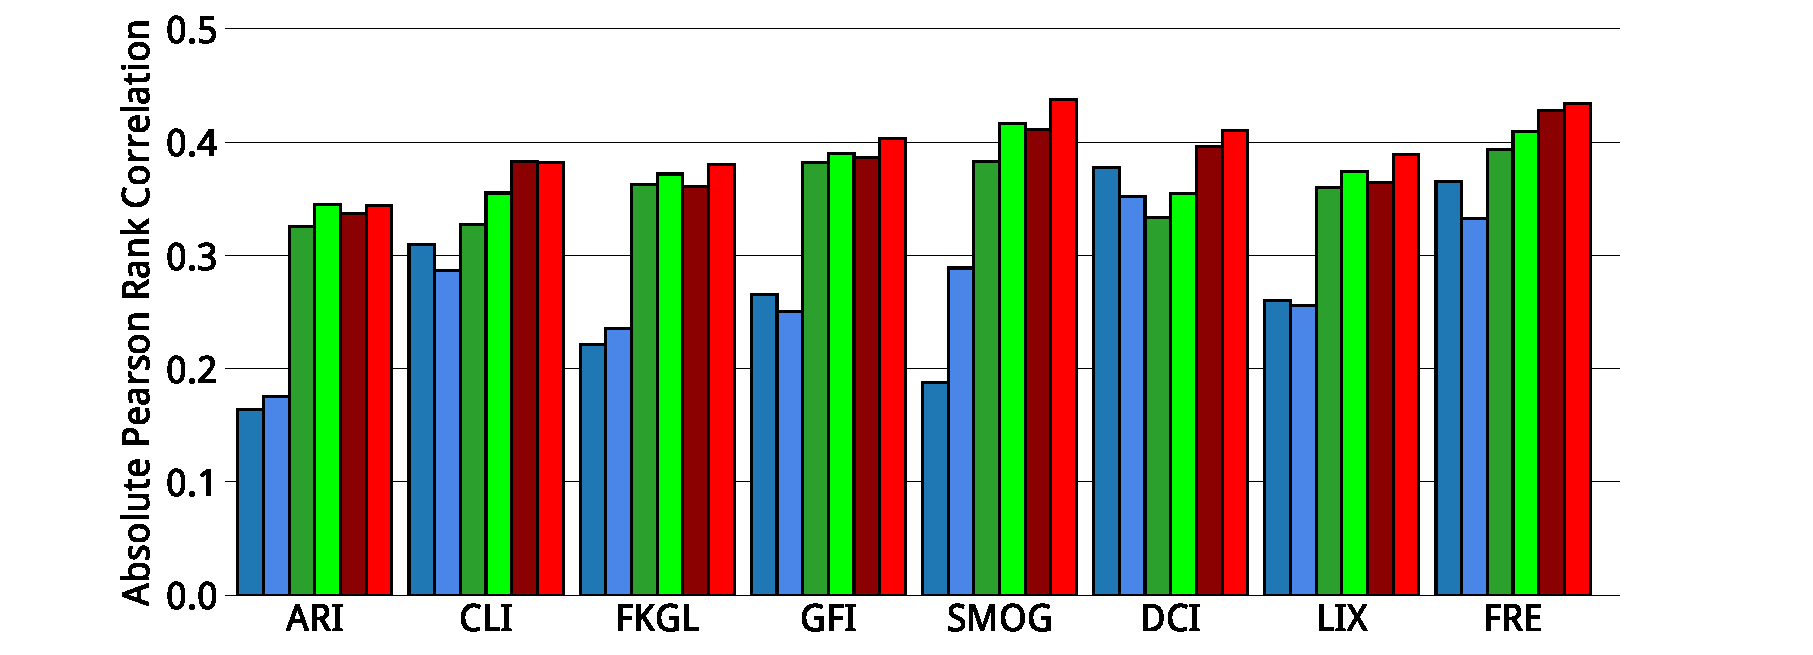
\includegraphics[width=1.\textwidth]{graphics/bar_corr_pearson15_values}
   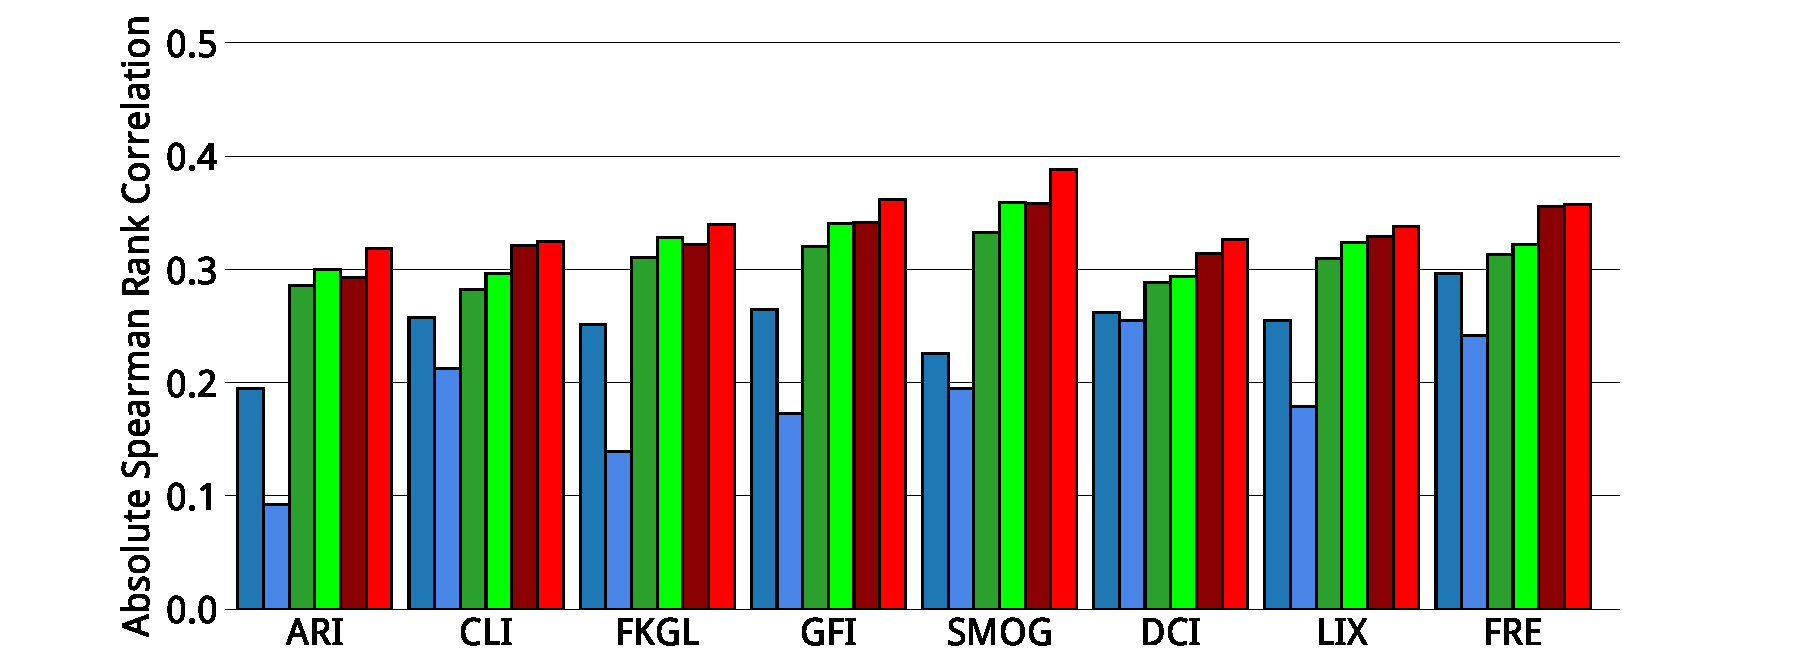
\includegraphics[width=1.00\textwidth]{graphics/bar_corr_spearman15_values}
   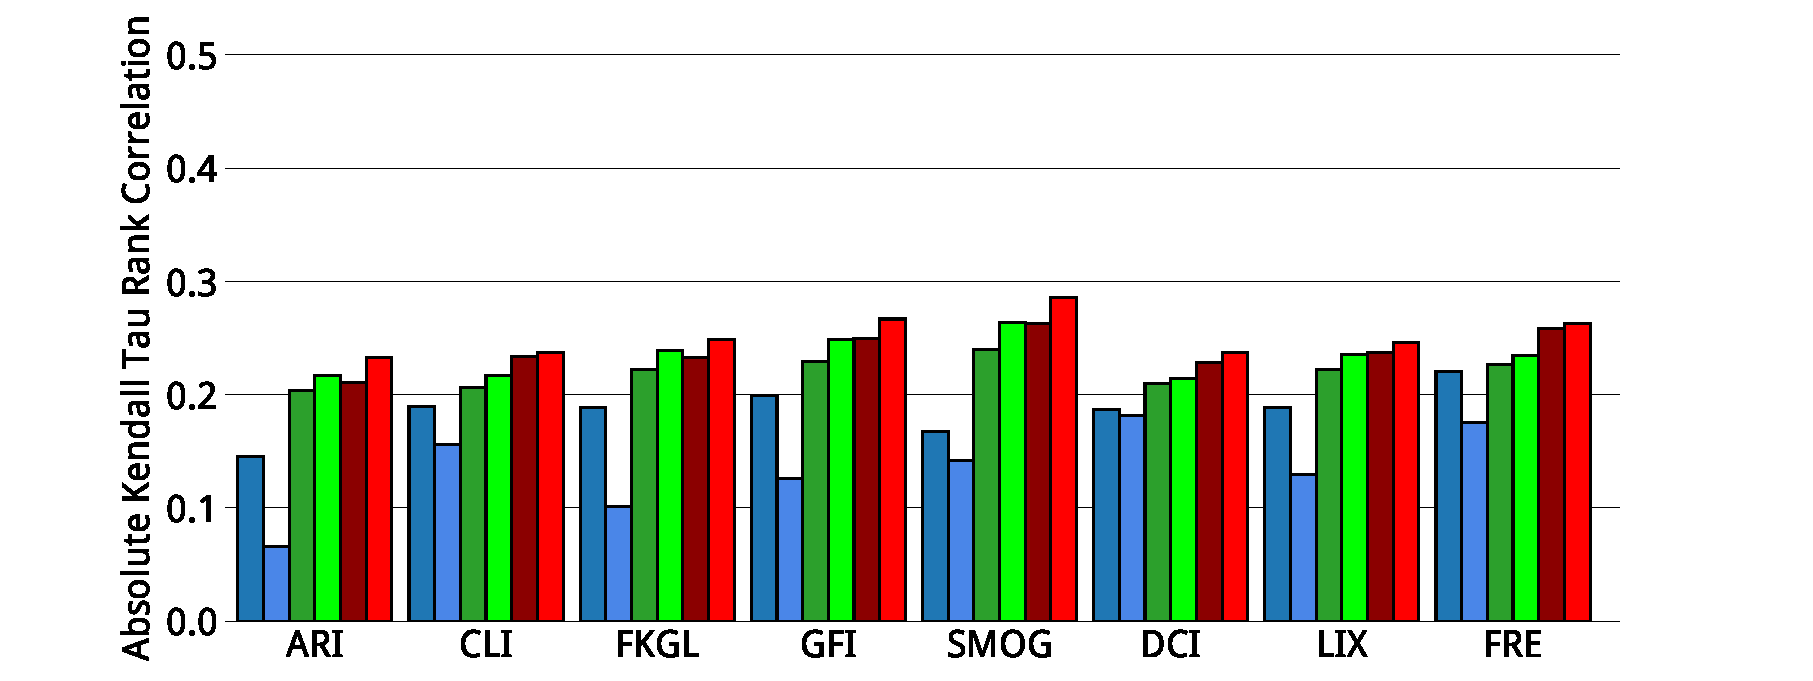
\includegraphics[width=1.00\textwidth]{graphics/bar_corr_kendalltau15_values}
   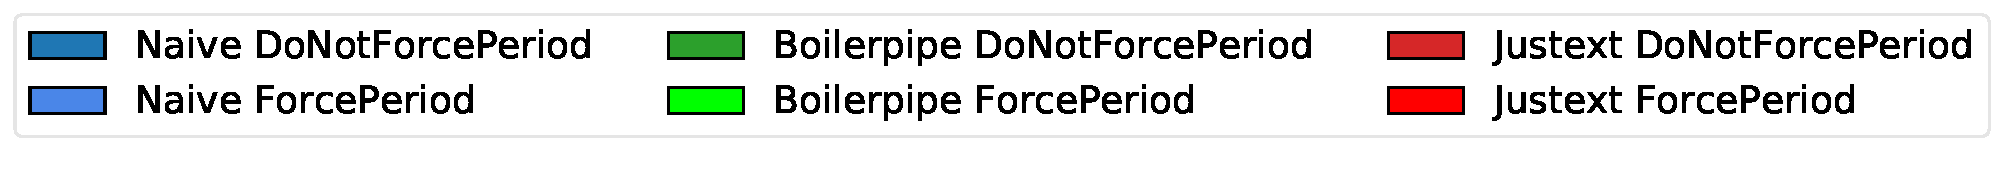
\includegraphics[width=1\textwidth]{graphics/legend62}
    \caption{Correlation of different readability measures and the understandability scores collected in CLEF eHealth 2015}
   \label{fig:bar_corr_clef15}
\end{figure}

\begin{figure}[th!]
   \centering
    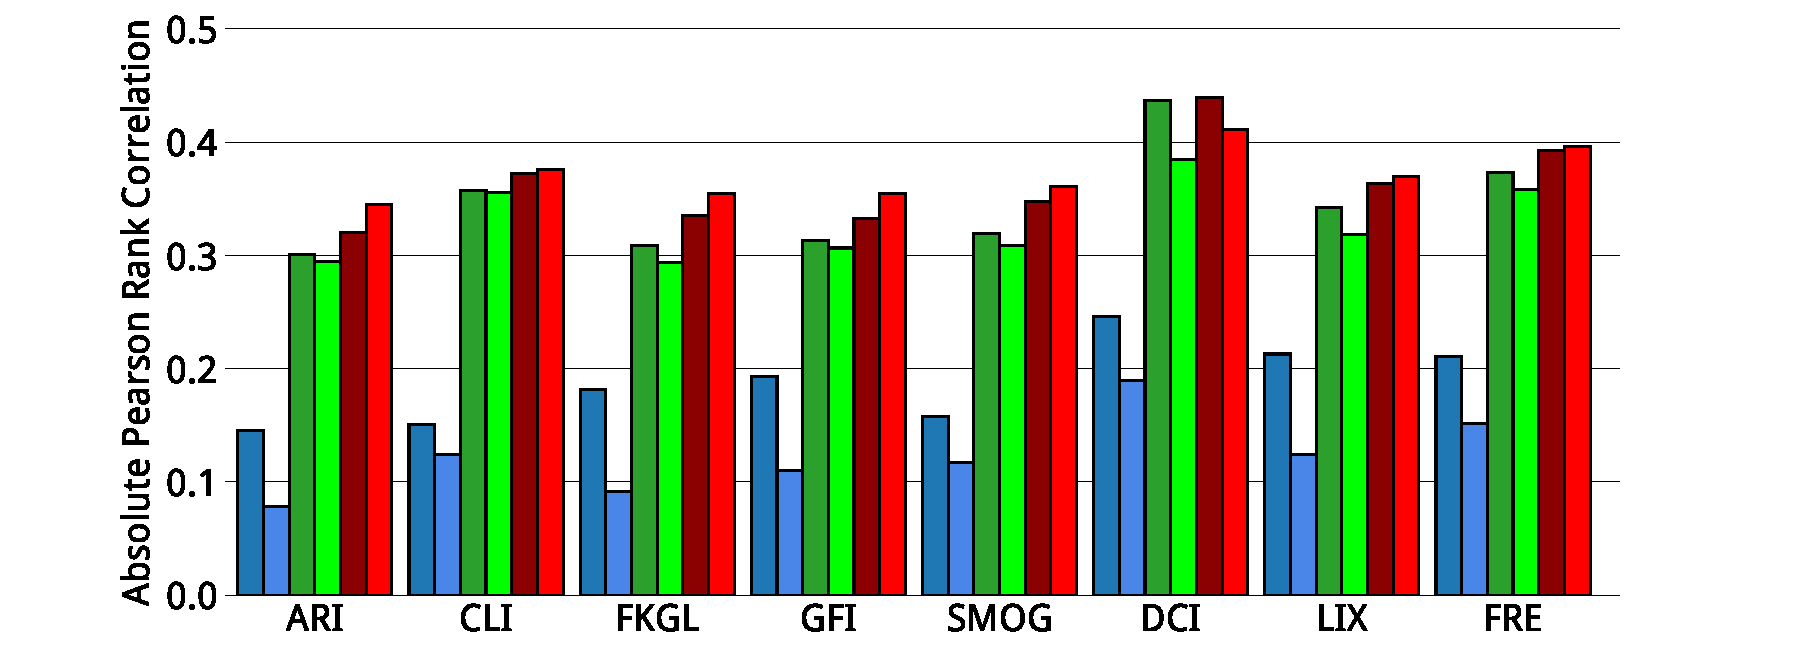
\includegraphics[width=1.\textwidth]{graphics/bar_corr_pearson16_values}
    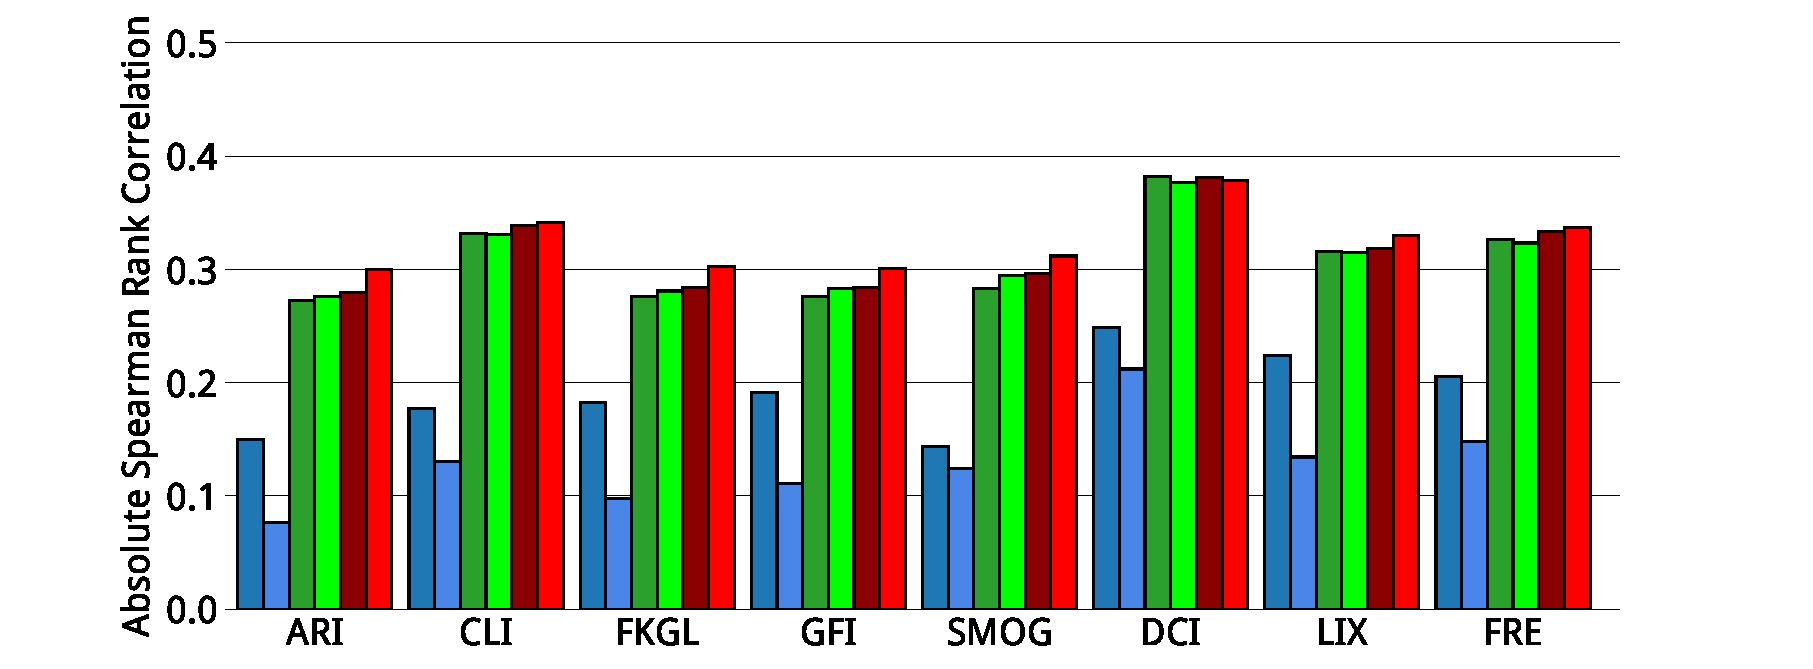
\includegraphics[width=1.\textwidth]{graphics/bar_corr_spearman16_values}
    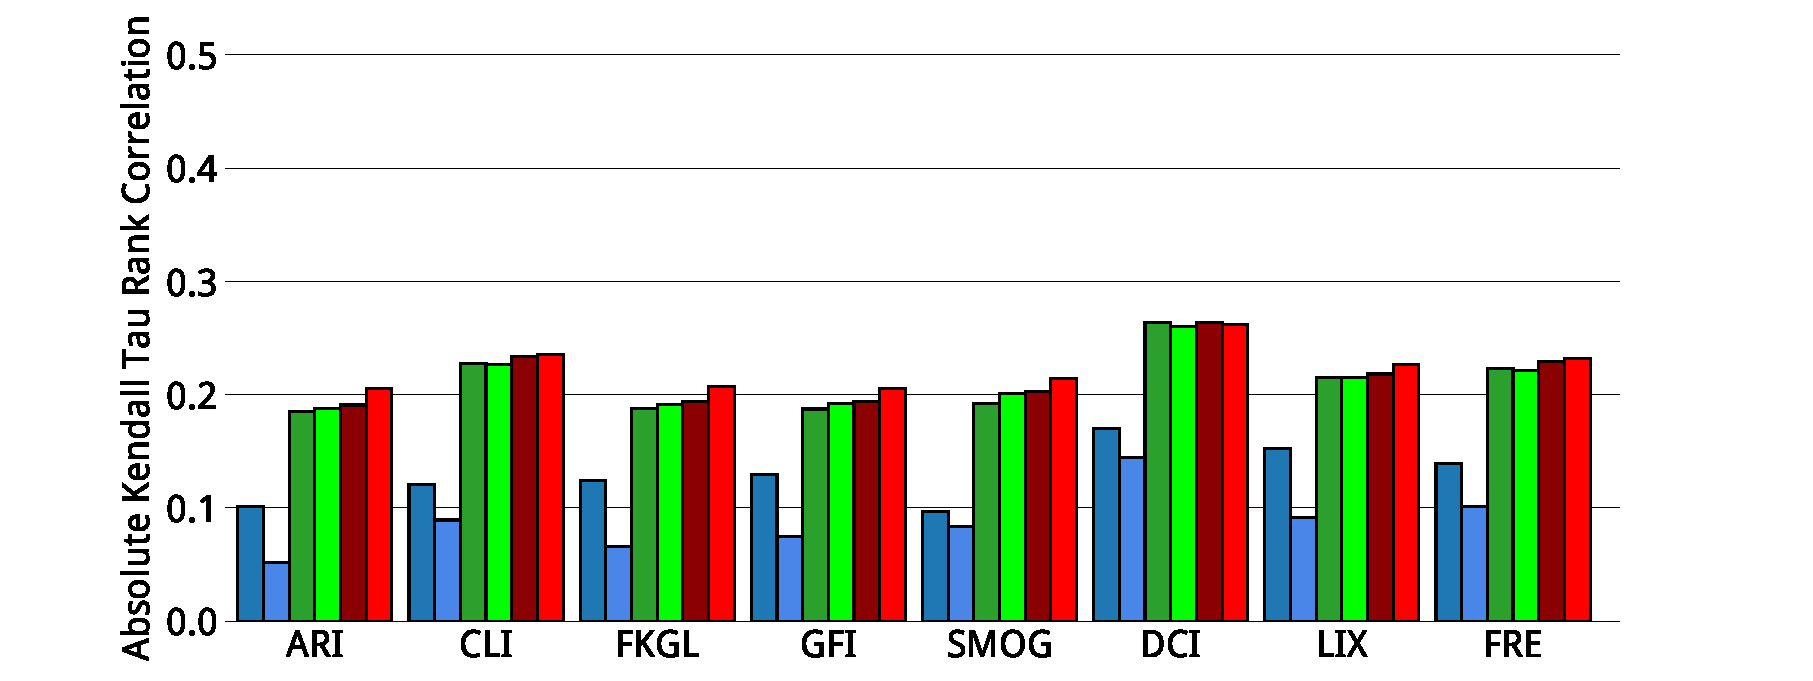
\includegraphics[width=1.\textwidth]{graphics/bar_corr_kendalltau16_values}
    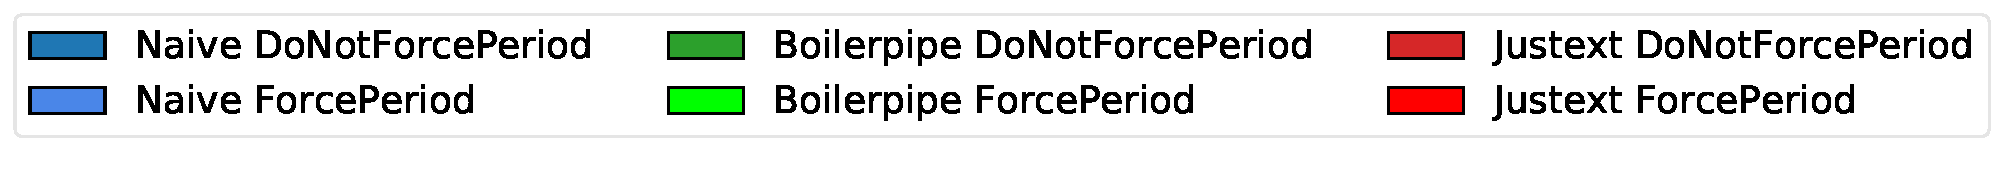
\includegraphics[width=1\textwidth]{graphics/legend62}
    \caption{Correlation of different readability measures and the understandability scores collected in CLEF eHealth 2016.}
   \label{fig:bar_corr_clef16}
\end{figure}


\section{(More) Understandability Estimators}
\label{sec:proxies}

The correlation of readability formulas as shown in Figures~\ref{fig:bar_corr_clef15} and~\ref{fig:bar_corr_clef16} is not strong, with no correlation being higher than 0.5.
One of our intents with the rest of this chapter is comparing the correlation of the traditional readability formulas with other methods for understandability estimation, including an evaluation of other  humans performing the same task.
For that, we devise and group several methods into semantically related groups which will be following presented.
We summarize all methods in Table~\ref{tab:doc_features}.

%Therefore, what unifies all methods listed in this section is the goal to automatically infer the understandability of a document, in our case, a Web page with medical content.
%For sake of understanding, in Table~\ref{tab:doc_features} we list all the methods used in this chapter to estimate document understandability.
%Note that we divide these estimators into semantically related groups, which are presented below.

\subsection{Traditional Readability Formulas}
This group contains all the readability formulas listed in Chapter~\ref{chp:preprocessing} (Table~\ref{tab:formulas}) and additional readability formulas that were excluded for not being on the same value scale as the other ones.

\subsection{Raw Components of Readability Formulas}
This group comprises the building blocks that make up the traditional readability measures. Some examples include the average number of characters per word or the average number of syllables in a sentence\footnote{Words were divided into syllables using the Python package Pyphen \url{http://pyphen.org/}}.

\subsection{General Medical Vocabularies}
This group includes methods such as the number of words with a medical prefix or suffix, i.e. beginning or ending with Latin or Greek particles (e.g., amni, angi, algia, arteri), acronyms \footnote{The acronym list was obtained from the ADAM database \cite{zhou2006}} or medical vocabularies such as the International Statistical Classification of Diseases and Related Health Problems (ICD), Drugbank and the OpenMedSpel dictionary\footnote{\url{http://extensions.openoffice.org/en/project/openmedspel-en-us}}. 
Methods listed here were matched with documents using a simple keywords matching.

\subsection{Consumer Vocabulary Features}
the Consumer Health Vocabulary (CHV) is a prominent medical vocabulary dedicated to mapping consumer (layperson) vocabulary to technical terms. 
It attributes a score for each of its concepts with respect to their difficulty, with lower/higher scores for harder/easier concepts.
We used MetaMap once again to map the content of Web documents, as done in Chapters~\ref{chp:user_query_logs} and~\ref{chp:medical_expertise}. 
We further use MetaMap options to also filter only concepts identified as symptoms or diseases, using the same definitions from Section~\ref{sec:semantic}. 
%The CHV dataset (version 20110204) links part of the UMLS concepts, such as “myocardial infarction”, to everyday expressions, “heart attack”.

\subsection{Expert Vocabulary Features}

The hierarchy of Medical Subject Headers (MeSH) was previously used in the literature to identify hard concepts, assuming that a concept that is deep in the hierarchy is harder than a shallow one~\cite{yan11}.
As done with CHV, we used MetaMap to map the content of Web documents to MeSH and explore symptoms and disease concepts separately.

\subsection{Natural Language}
This group comprises commonly used metrics in the natural language processing field: the ratio of part-of-speech (POS) classes, the number of entities in a text, the sentiment polarity and the ratio of words found in English vocabularies. The Python package NLTK 3.2\footnote{\url{http://www.nltk.org/}} was employed for sentiment analysis and POS tagging. The GNU Aspell\footnote{\url{http://www.aspell.net/}} dictionary was used as a standard English vocabulary and a stopword list was built by merging the stopword
lists of the Indri\footnote{\url{http://www.lemurproject.org/indri/}} and Terrier\footnote{\url{http://www.terrier.org/}} toolkits. 

\subsection{HTML Features}
The aim of this group is to represent a web page by its HTML content.
We hypothesize that a Web page rich of images or with its content well summarized in tables can potentially ease hard subjects such as medicine. 
We identify a large number of HTML tags in this group with the Python library BeautifulSoap v4.4\footnote{\url{https://www.crummy.com/software/BeautifulSoup/}}.

\subsection{Word Frequency Features}
\label{sec:word_freq}

Common and known words are usually frequent words, while unknown and obscure words are rare. This idea is implemented in readability formulas such as the Dale-Chall index which uses a list of common words and counts the number of words that fall outside this list~\cite{dale48}.
In this work we model word frequency in a straightforward manner: we sort the frequency of all words in a corpus and normalize the ranking of word frequency such that values close to 100 are attributed to common words and values close to 0 to rare words. 
We explore three different corpora in this work:

\begin{itemize}
\item Medical Reddit: Reddit is an Internet forum with a sizable user community which is responsible for generating content. Any user can start a discussion receiving replies from any other user.
This discussion forum is intensively used for health purposes, for example in the Reddit community AskDocs licensed nursers and doctors (subject to user identity verification) advise help seekers free of charge. We selected six of such communities (medical, AskDocs, AskDoctorSmeeee, Health, WomensHealth, Mens\_Health) and downloaded all user interactions using the Python Reddit API Wrapper (PRAW\footnote{\url{https://praw.readthedocs.io/}}), v5.1. In total 43,018 discussions were collected.

\item PubMed Central: PubMed Central (PMC) is an online digital database of freely available full-text biomedical literature playing a similar role to physicians as the ACM Digital Library does to computer scientists. We used in this work the same collection crafted for the TREC Clinical Decision Support Track 2014 and 2015 (TREC-CDS)\footnote{\url{http://www.trec-cds.org/}} consisting of 733,138 articles. 
 
\item Medical English Wikipedia: we filtered articles from a Wikipedia dump\footnote{\url{https://dumps.wikimedia.org/enwiki/}} (May 1st 2017), that contained an Infobox\footnote{A Wikipedia infobox is a template containing structured information that appear on the right of Wikipedia pages to summarize key aspects of concepts} in which at least one of the following words appeared as a property: ICD10, ICD9, DiseasesDB, MeSH, MeSHID, MeshName, MeshNumber, GeneReviewsName, Orphanet, eMedicine, MedlinePlus, drug\_name, Drugs.com, DailyMedID, LOINC.
Figure~\ref{fig:hyperthermia} illustrates a Wikipedia page that is marked as medical because of its Infobox entries.
This idea was successfully implemented in Soldaini et al.~\cite{soldaini15} and our filtering process resulted in a collection of 11,942 articles. 
Note that this procedure highly favors precision over recall.
   
\end{itemize}

A summary of the statistics of these three collections is reported in Table~\ref{tab:collection_stats}.
In order to calculate word frequency, we removed words that occur less than 5 times in a corpus.
Finally, we ignore out of vocabulary (OV) words in our calculations, unless it is explicitly stated.

\begin{figure}[th!]
   \centering
   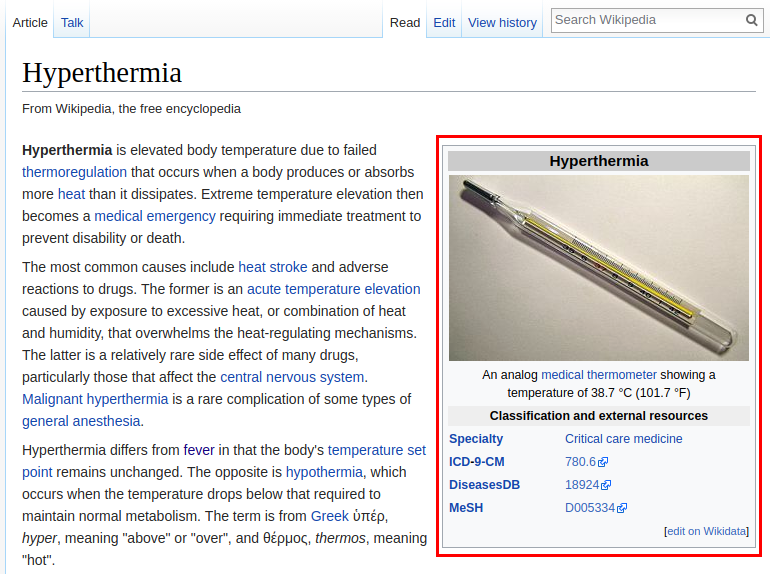
\includegraphics[width=1.00\textwidth]{graphics/hyperthermia}
    \caption{Wikipedia page on hyperthermia. A rectangular red box identify the Infobox on the right hand side containing entries for Specialty, ICD-9-CM, DiseasesDB and MeSH.}
    \label{fig:hyperthermia}
\end{figure}

\begin{table}[!tb]
\centering    
\caption{Statistics for the collections used as background models for understandability estimations.}
\vspace{-0.3cm}
\label{tab:collection_stats}
\resizebox{0.4\textwidth}{!}{
\begin{tabular}{cccc}
\toprule 
\textbf{Statistic} & \textbf{Medical Wikipedia} & \textbf{Medical Reddit} & \textbf{PubMed Central}\tabularnewline
\midrule 
\textbf{Number of Docs.} & 11,868 & 43,019 & 733,191\tabularnewline
\textbf{Number of Words} & 10,655,572 & 11,978,447 & 144,024,976\tabularnewline
\textbf{Number of Unique Words} & 467,650 & 317,106 & 2,933,167\tabularnewline
\textbf{Avg. Words per Doc.} & 898.90 $\pm$ 1351.76 & 278.45 $\pm$ 359.70  & 227.22 $\pm$ 270.44 \tabularnewline
\textbf{Avg. Char per Doc.} & 5107.81 $\pm$ 7618.57  & 1258.44 $\pm$ 1659.96  & 1309.11 $\pm$ 1447.31 \tabularnewline
\textbf{Avg. Char per Word} & 5.68 $\pm$ 3.75  & 4.52 $\pm$ 3.52 &  5.76 $\pm$ 3.51 \tabularnewline
\bottomrule
\end{tabular}
} % End of resizebox
\vspace{-8pt}
\end{table}


\subsection{Machine Learning on Text - Regressors and Classifiers}

In a recent survey, Kevin Collins-Thompson reports that the future of understandability estimation relies on Machine Learning~\cite{collins2014computational}.
A challenge in using Machine Learning in this task is defining the background corpora used as training set.
A possible setup for our work could have used CLEF 2015 assessments to learn a model for CLEF 2016 and vice-versa, but instead, we opt for a 
more reusable solution for the medical/health domain. 
We employed the three datasets explained in Section~\ref{sec:word_freq} and assume different labels according to the average difficulty of documents in these collections:

\begin{itemize}
    \item Medical Reddit (label 1): Documents in this collection are expected to be written in a colloquial style, and thus the easiest to understand. All the conversations are in fact explicitly directed to assist inexpert health consumers;
    \item Medical English Wikipedia (label 2): Documents in this collection are expected to be less formal than scientific articles, but more formal than a Web forum like Reddit;
    \item PubMed Central (label 3): Documents from this collection are expected to be written in a highly formal style, as the target audience of these documents are physicians, nursers and researchers in the biomedical domain.
\end{itemize}

Based on word counts in documents in these three collections, we model two different tasks a classification one and a regression task.
Different labels for the regression could be employed, for example, a label 5 to PubMed Central documents to emphasize that these documents are explicitly made for expert users.
We did not explore the effects of different labels in this work, it is left as future work.

\begin{table*}[tb]
\caption{Metrics used as understandability proxies; $\star$: raw values are used. $\diamondsuit$: values normalised by number of words in a documents are used. $\dagger$: values normalised by number of sentences in a document are used.}
\label{tab:doc_features}
\resizebox{1.\textwidth}{!}{
\begin{tabular}{llcll}
\cline{1-2} \cline{4-5} 
\textbf{Group} & \textbf{Metric} & \multirow{29}{*}{} & \textbf{Group} & \textbf{Metric}\tabularnewline
\cline{1-2} \cline{4-5} 
\multirow{8}{*}{\textbf{Traditional Readability Formulas}} & Automated Readability Index (ARI) \cite{ari67} &  & \multirow{26}{*}{\textbf{HTML Features}} & \# of Abbr tags\tabularnewline
 & Coleman-Liau Index (CLI) \cite{cli75} &  &  & \# of A tags\tabularnewline
 & Dale Chall Index (DCI) \cite{dale48} &  &  & \# of Blockquote tags\tabularnewline
 & Flesch-Kincaid Grade Level (FKGL) \cite{flesch75} &  &  & \# of Bold tags\tabularnewline
 & Flesch Reading Ease (FRE) \cite{flesch75} &  &  & \# of Cite tags\tabularnewline
 & Gunning Fog Index (GFI) \cite{gunning52} &  &  & \# of Div tags\tabularnewline
 & Lasbarhetsindex (LIX) \cite{lix} &  &  & \# of Forms tags\tabularnewline
 & Simple Measure of Gobbledygook (SMOG) \cite{smog69} &  &  & \# of H1 tags\tabularnewline
\cline{1-2} 
\multirow{10}{*}{\textbf{\makecell{\kern-2.8emRaw Components \\of Readability Measures}}} & \# of Characters $^{\star\diamondsuit\dagger}$ &  &  & \# of H2 tags\tabularnewline
 & \# of Words $^{\star\dagger}$ &  &  & \# of H3 tags\tabularnewline
 & \# of Sentences {$^{\star\diamondsuit}$} &  &  & \# of H4 tags\tabularnewline
 & \# of Difficult Words (Dale Chall list \cite{dale48})
$^{\star\diamondsuit\dagger}$ &  &  & \# of H5 tags\tabularnewline
 & \# of Words Longer than 4 chars $^{\star\diamondsuit\dagger}$ &  &  & \# of H6 tags\tabularnewline
 & \# of Words Longer than 6 chars $^{\star\diamondsuit\dagger}$ &  &  & \# of Hs (any H above)\tabularnewline
 & \# of Words Longer than 10 chars $^{\star\diamondsuit\dagger}$ &  &  & \# of Img tags\tabularnewline
 & \# of Words Longer than 13 chars $^{\star\diamondsuit\dagger}$ &  &  & \# of Input tags\tabularnewline
 & \# of Number of Syllables $^{\star\diamondsuit\dagger}$ &  &  & \# of Link tags\tabularnewline
 & \# of Polysyllable Words (>3 Syllables) $^{\star\diamondsuit\dagger}$ &  &  & \# of DL tags\tabularnewline
\cline{1-2} 
\multirow{6}{*}{\textbf{Medical Vocabularies}} & \# of Words with Medical Prefix $^{\star\diamondsuit\dagger}$ &  &  & \# of UL tags\tabularnewline
 & \# of Words with Medical Suffix $^{\star\diamondsuit\dagger}$ &  &  & \# of OL tags\tabularnewline
 & \# of Acronyms $^{\star\diamondsuit\dagger}$ &  &  & \# of List (DL + UL + OL)\tabularnewline
 & \# of ICD Concepts $^{\star\diamondsuit\dagger}$ &  &  & \# of Q tags\tabularnewline
 & \# of Drugbank $^{\star\diamondsuit\dagger}$ &  &  & \# of Scripts tags\tabularnewline
 & \# of Words in medical dict. (OpenMedSpel) $^{\star\diamondsuit\dagger}$ &  &  & \# of Spans tags\tabularnewline
\cline{1-2} 
    \multirow{6}{*}{\textbf{\makecell{\kern-2.5emConsumer Health\\ Vocabulary (CHV) \cite{zeng06} \\ \kern-6.2emFeatures}}} & CHV Mean Score for all Concepts $^{\star\diamondsuit\dagger}$ &  &  & \# of Table tags\tabularnewline
 & \# of CHV Concepts $^{\star\diamondsuit\dagger}$ &  &  & \# of P tags\tabularnewline
\cline{4-5} 
 & CHV Mean Score for Symptom Concepts $^{\star\diamondsuit\dagger}$ &  & \multirow{20}{*}{\textbf{Word Frequency}} & 25th percentil English Wikipedia\tabularnewline
 & \# of CHV Symptom Concepts $^{\star\diamondsuit\dagger}$ &  &  & 50th percentil English Wikipedia\tabularnewline
 & CHV Mean Score for Disease Concepts $^{\star\diamondsuit\dagger}$ &  &  & 75th percentil English Wikipedia\tabularnewline
 & \# of CHV Disease Concepts $^{\star\diamondsuit\dagger}$ &  &  & Mean Rank English Wikipedia\tabularnewline
\cline{1-2} 
\multirow{6}{*}{\textbf{\makecell{\kern-0.3emMedical Subject\\ Headers (MeSH)}}} & \# of MeSH Concepts $^{\star\diamondsuit\dagger}$ &  &  & Mean Rank English Wikipedia - Includes OV\tabularnewline
 & Average Tree of MeSH Concepts $^{\star\diamondsuit\dagger}$ &  &  & 25th percentil Medical Reddit\tabularnewline
 & \# of MeSH Symptom Concepts $^{\star\diamondsuit\dagger}$ &  &  & 50th percentil Medical Reddit\tabularnewline
 & Average Tree of MeSH Symptom Concepts $^{\star\diamondsuit\dagger}$ &  &  & 75th percentil Medical Reddit\tabularnewline
 & \# of MeSH Disease Concepts $^{\star\diamondsuit\dagger}$ &  &  & Mean Rank Medical Reddit\tabularnewline
 & Average Tree of MeSH Disease Concepts $^{\star\diamondsuit\dagger}$ &  &  & Mean Rank Medical Reddit ncludelude OV\tabularnewline
\cline{1-2} 
\multirow{20}{*}{\textbf{Natural Language}} & Positive Words $^{\star\diamondsuit\dagger}$ &  &  & 25th percentil Pubmed\tabularnewline
 & Negative Words $^{\star\diamondsuit\dagger}$ &  &  & 50th percentil Pubmed\tabularnewline
 & Neutral Words $^{\star\diamondsuit\dagger}$ &  &  & 75th percentil Pubmed\tabularnewline
 & \# of verbs $^{\star\diamondsuit\dagger}$ &  &  & Mean Rank Pubmed\tabularnewline
 & \# of nouns $^{\star\diamondsuit\dagger}$ &  &  &  Mean Rank Pubmed - Includes OV\tabularnewline
 & \# of pronouns $^{\star\diamondsuit\dagger}$ &  &  & 25th p. Wikipedia+Reddit+Pubmed  \tabularnewline
 & \# of adjectives $^{\star\diamondsuit\dagger}$ &  &  & 50th p. Wikipedia+Reddit+Pubmed \tabularnewline
 & \# of adverbs $^{\star\diamondsuit\dagger}$ &  &  & 75th p. Wikipedia+Reddit+Pubmed \tabularnewline
 & \# of adpositions $^{\star\diamondsuit\dagger}$ &  &  & Mean R. Wiki.+Reddit+Pubmed \tabularnewline 
 & \# of conjunctions $^{\star\diamondsuit\dagger}$ & &  & Mean R. Wiki.+Reddit+Pubmed - w. OV \tabularnewline
\cline{4-5} 
 & \# of determiners $^{\star\diamondsuit\dagger}$ & & \multirow{5}{*}{\textbf{Regressor}} & Linear Regressor\tabularnewline  
 & \# of cardinal numbers $^{\star\diamondsuit\dagger}$ &  &  & Gradient Boosting Regressor\tabularnewline
 & \# of particles or other function words $^{\star\diamondsuit\dagger}$ &  &  & Multi-layer Perceptron Regressor\tabularnewline
 & \# of other POS (foreign words, typos) $^{\star\diamondsuit\dagger}$ &  &  & Random Forest Regressor\tabularnewline
 & \# of punctuation $^{\star\diamondsuit\dagger}$ &  &  & Support Vector Machine Regressor\tabularnewline
\cline{4-5} 
 & Height of part-of-speech parser tree $^{\star\diamondsuit\dagger}$ &  &  \multirow{6}{*}{\textbf{Classifier}} & Logistic Regression\tabularnewline
 & \# of Entities $^{\star\diamondsuit\dagger}$ &  &  & Gradient Boosting Classifier\tabularnewline
 & \# of Stopwords $^{\star\diamondsuit\dagger}$ &  &  & Multinomial Naive Bayes\tabularnewline
 & \# of words not found in Aspell Eng. dict. $^{\star\diamondsuit\dagger}$ &  &  & Multi-layer Perceptron Classifier\tabularnewline
 &  &  &  & Random Forest Classifier\tabularnewline
 &  &  &  & Support Vector Machine Classifier\tabularnewline
\cline{1-2} \cline{4-5} 
\end{tabular}
}
\end{table*}


\section{Top Measures from Each Group}
\label{sec:beyond_readability}

We correlated each individual understandability estimator listed in Table~\ref{tab:doc_features} with the human assessments collected in CLEF eHealth 2015 and 2016 campaigns.
We report in Table~\ref{tab:top_corr_metrics} the best metric for each group according to Pearson, Spearman or Kendall correlation.
For some groups, such as the readability formula group, the highest correlated metric was the same for different correlation measure: SMOG Index in CLEF eHealth 2015 and Dale-Chall Index in 2016. 
We highlight the top score value of each correlation measure in each group. Note that there is no single case in which three different metrics were the top correlated for each different correlation measure.
\todo{hypotesis that kendatll tau and spearman always point to the same winner}

Interestingly, Table~\ref{tab:top_corr_metrics} shows that the polysyllable words, best formula component metric for CLEF 2015 data, is the main metric for the SMOG formula, the best readability formula for CLEF 2015. 
Likewise, the number of difficult words, best formula component metric for CLEF 2016, is the main metric for Dale-Chall index, the best readability formula for CLEF 2016.

The top correlation for MeSH group, number of MeSH concepts, reaches much lower correlation than the top correlation metric for the CHV group, the scores of CHV concepts.
The dominating metrics for the Natural Language group are the number of pronouns, the number of stopwords and the number of out of vocabulary words; all these are consistently more correlated than metrics in the MeSH and CHV group.
In turn, the top correlations for the HTML group, counts of P tags and list tags, were the weakest. P tags are used to create paragraphs in a Web page, being roughly a proxy for text lengthiness. 
Top estimators for the word frequency group are based on the Medical Reddit and PubMed counts, with correlations as high as the readability formulas.
Finally, the group with the highest correlated estimators are the regressors and classifiers, with top estimators being the Neural Network regressor and the multinomial Naive Bayes.
\todo{this section misses some short of conclusion or at least a link to the next section}
%
\begin{table}[t]
\centering    
\caption{Metrics with highest correlation per group. In bold are the metric that archived the highest correlation for a correlation measure.}
\label{tab:top_corr_metrics}
\resizebox{.45\textwidth}{!}{ %%%%
\begin{tabular}{c|c|c|c|c|c|c}
\toprule
\textbf{Dataset} & \textbf{Group} & \textbf{Metric} & \textbf{Preproc.} & \textbf{Pears.} & \textbf{Spear.} & \textbf{Kend.}\tabularnewline
\midrule
\multirow{15}{*}{CLEF 2015} & RF & SMOG Index & JST NFP & \textbf{0.438} & \textbf{0.388} & \textbf{0.286}\tabularnewline
\cmidrule{2-7} 
 & \multirow{2}{*}{CRF} & Avg. Num. of Polysyl. Words per Word & JST FP & \textbf{0.429} & 0.364 & 0.268\tabularnewline
 &  & Avg. N. of Polysyl. Words per Sentence & JST NFP & 0.192 & \textbf{0.388} & \textbf{0.286}\tabularnewline
\cmidrule{2-7} 
& \multirow{2}{*}{GMV} & Avg. N. Medical Prefixes per Word & Naive FP & \textbf{0.314} & 0.312 & 0.229\tabularnewline
 &  & Number of Medical Prefixes & Naive FP & 0.131 & \textbf{0.368} & \textbf{0.272}\tabularnewline
\cmidrule{2-7} 
 & CMV & CHV Mean Score for all Concepts & Naive FP & \textbf{0.371} & \textbf{0.314} & \textbf{0.228}\tabularnewline
\cmidrule{2-7} 
 & EMV & Number of MeSH Concepts & Naive FP & \textbf{0.227} & \textbf{0.249} & \textbf{0.178}\tabularnewline
\cmidrule{2-7} 
 &  \multirow{2}{*}{NLF} & N. of words not found in Aspell Dict. & JST NFP & \textbf{0.351} & 0.276 & 0.203\tabularnewline
 &  & Number of Pronouns per Word & Naive FP & 0.271 & \textbf{0.441} & \textbf{0.325}\tabularnewline
\cmidrule{2-7} 
 & HF & Number of P Tags & None & \textbf{0.219} & \textbf{0.196} & \textbf{0.142}\tabularnewline
\cmidrule{2-7} 
 &  \multirow{2}{*}{WFF} & Mean Rank Medical Reddit - Includes OV & JST NFP & \textbf{0.435} & 0.277 & 0.197\tabularnewline
 &  & 25th percentil Pubmed & JST NFP & 0.330 & \textbf{0.347} & \textbf{0.256}\tabularnewline
\cmidrule{2-7} 
 &  \multirow{2}{*}{MLR} & Neural Network Regressor & BOI NFP & \textbf{0.602} & 0.394 & 0.287\tabularnewline
 &  & Neural Network Regressor & JST FP & 0.565 & \textbf{0.438} & \textbf{0.324}\tabularnewline
\cmidrule{2-7} 
 & MLC & Multinomial Naive Bayes & Naive FP & \textbf{0.573} & \textbf{0.477} & \textbf{0.416}\tabularnewline
\midrule
\midrule
\multirow{18}{*}{CLEF 2016} & \multirow{2}{*}{RF} & Dale Chall Index & JST FP & \textbf{0.439} & 0.381 & 0.264\tabularnewline
 &  & Dale Chall Index & BOI FP & 0.437 & \textbf{0.382} & \textbf{0.264}\tabularnewline
\cmidrule{2-7} 
 & CRF & Avg. Difficult Words Per Word & BOI FP & \textbf{0.431} & \textbf{0.379} & \textbf{0.262}\tabularnewline
\cmidrule{2-7} 
 & \multirow{2}{*}{GMV} & Avg. Prefixes per Sentence & JST FP & \textbf{0.263} & 0.242 & 0.164\tabularnewline
 &  & ICD Concepts Per Sentence & JST NFP & 0.014 & \textbf{0.253} & \textbf{0.172}\tabularnewline
\cmidrule{2-7} 
 & \multirow{2}{*}{CMV} & CHV Mean Score for all Concepts & JST FP & \textbf{0.329} & 0.313 & 0.216\tabularnewline
 &  & CHV Mean Score for all Concepts & BOI FP & 0.329 & \textbf{0.325} & \textbf{0.224}\tabularnewline
\cmidrule{2-7} 
 & \multirow{2}{*}{EMV} & Number of MeSH Concepts & BOI NFP & \textbf{0.201} & 0.166 & 0.113\tabularnewline
 &  & Number of MeSH Disease Concepts & BOI NFP & 0.179 & \textbf{0.192} & \textbf{0.132}\tabularnewline
\cmidrule{2-7} 
 & \multirow{2}{*}{NLF} & Avg. Stopword Per Word & BOI FP & \textbf{0.344} & 0.312 & 0.213\tabularnewline
 &  & Number of Pronouns & BOI FP & 0.341 & \textbf{0.364} & \textbf{0.252}\tabularnewline
\cmidrule{2-7} 
& \multirow{2}{*}{HF} & Number of Lists & \multirow{2}{*}{None} & \textbf{0.114} & 0.021 & 0.015\tabularnewline
 &  & Number of P Tags &  & 0.110 & \textbf{0.123} & \textbf{0.084}\tabularnewline
\cmidrule{2-7} 
 & \multirow{2}{*}{WFF} & Mean Rank Medical Reddit & BOI NFP & \textbf{0.387} & 0.312 & 0.214\tabularnewline
 &  & 50th percentil Medical Reddit & JST NFP & 0.351 & \textbf{0.315} & \textbf{0.216}\tabularnewline
\cmidrule{2-7} 
 & \multirow{2}{*}{MLR} & Neural Network Regressor & JST NFP & \textbf{0.454} & \textbf{0.373} & 0.258\tabularnewline
 &  & Random Forest Regressor & BOI NFP & 0.389 & 0.355 & \textbf{0.264}\tabularnewline
\cmidrule{2-7} 
 & MLC & Multinomial Naive Bayes & JST FP & \textbf{0.461} & \textbf{0.391} & \textbf{0.318}\tabularnewline
\bottomrule
\end{tabular}
} %%%%% ---- 
\end{table}

%

\section{Which Preprocessing Approach To Prefer}
\label{sec:which_preprocessing}

We further investigate the preprocessing steps with the groups of features introduced in Table~\ref{tab:doc_features}.
For that, we present in Figures~\ref{fig:boxplot_corr_docs_2015} and~\ref{fig:boxplot_corr_docs_2016} the box plot of different correlation metrics divided by preprocessing alternative for CLEF eHealth 2015 and 2016. 
For instance, the very first box plot in the upper part of these figures shows the absolute Pearson's rank correlation of different readability metrics when using a combination of Naive and ForcePeriod as preprocessing steps.
Boxes extend from the lower to upper quartile values of the data, with a line at the median. Whiskers extend from the box to show the range of the data. Flier points are those past the end of the whiskers, usually interpreted as outlier values.

We also include in Figures~\ref{fig:boxplot_corr_docs_2015} and~\ref{fig:boxplot_corr_docs_2016} boxes for the summary of the 3 preprocessing procedures to remove HTML, the use of HTML features, which is done without any preprocessing and the comparison with other human assessors. For CLEF eHealth 2015, we used as human assessments the additional assessments made by unpaid medical students and health consumers (see~\cite{palotti16b}), while for CLEF eHealth 2016 data, we randomly selected 100 pages that were assessed by another assessor. \mytodo{add at least another person doing assessments}.
The correlations with human assessments provide important insights on how hard and subjective understandability assessments are.

\begin{figure}[th!]
   \centering
   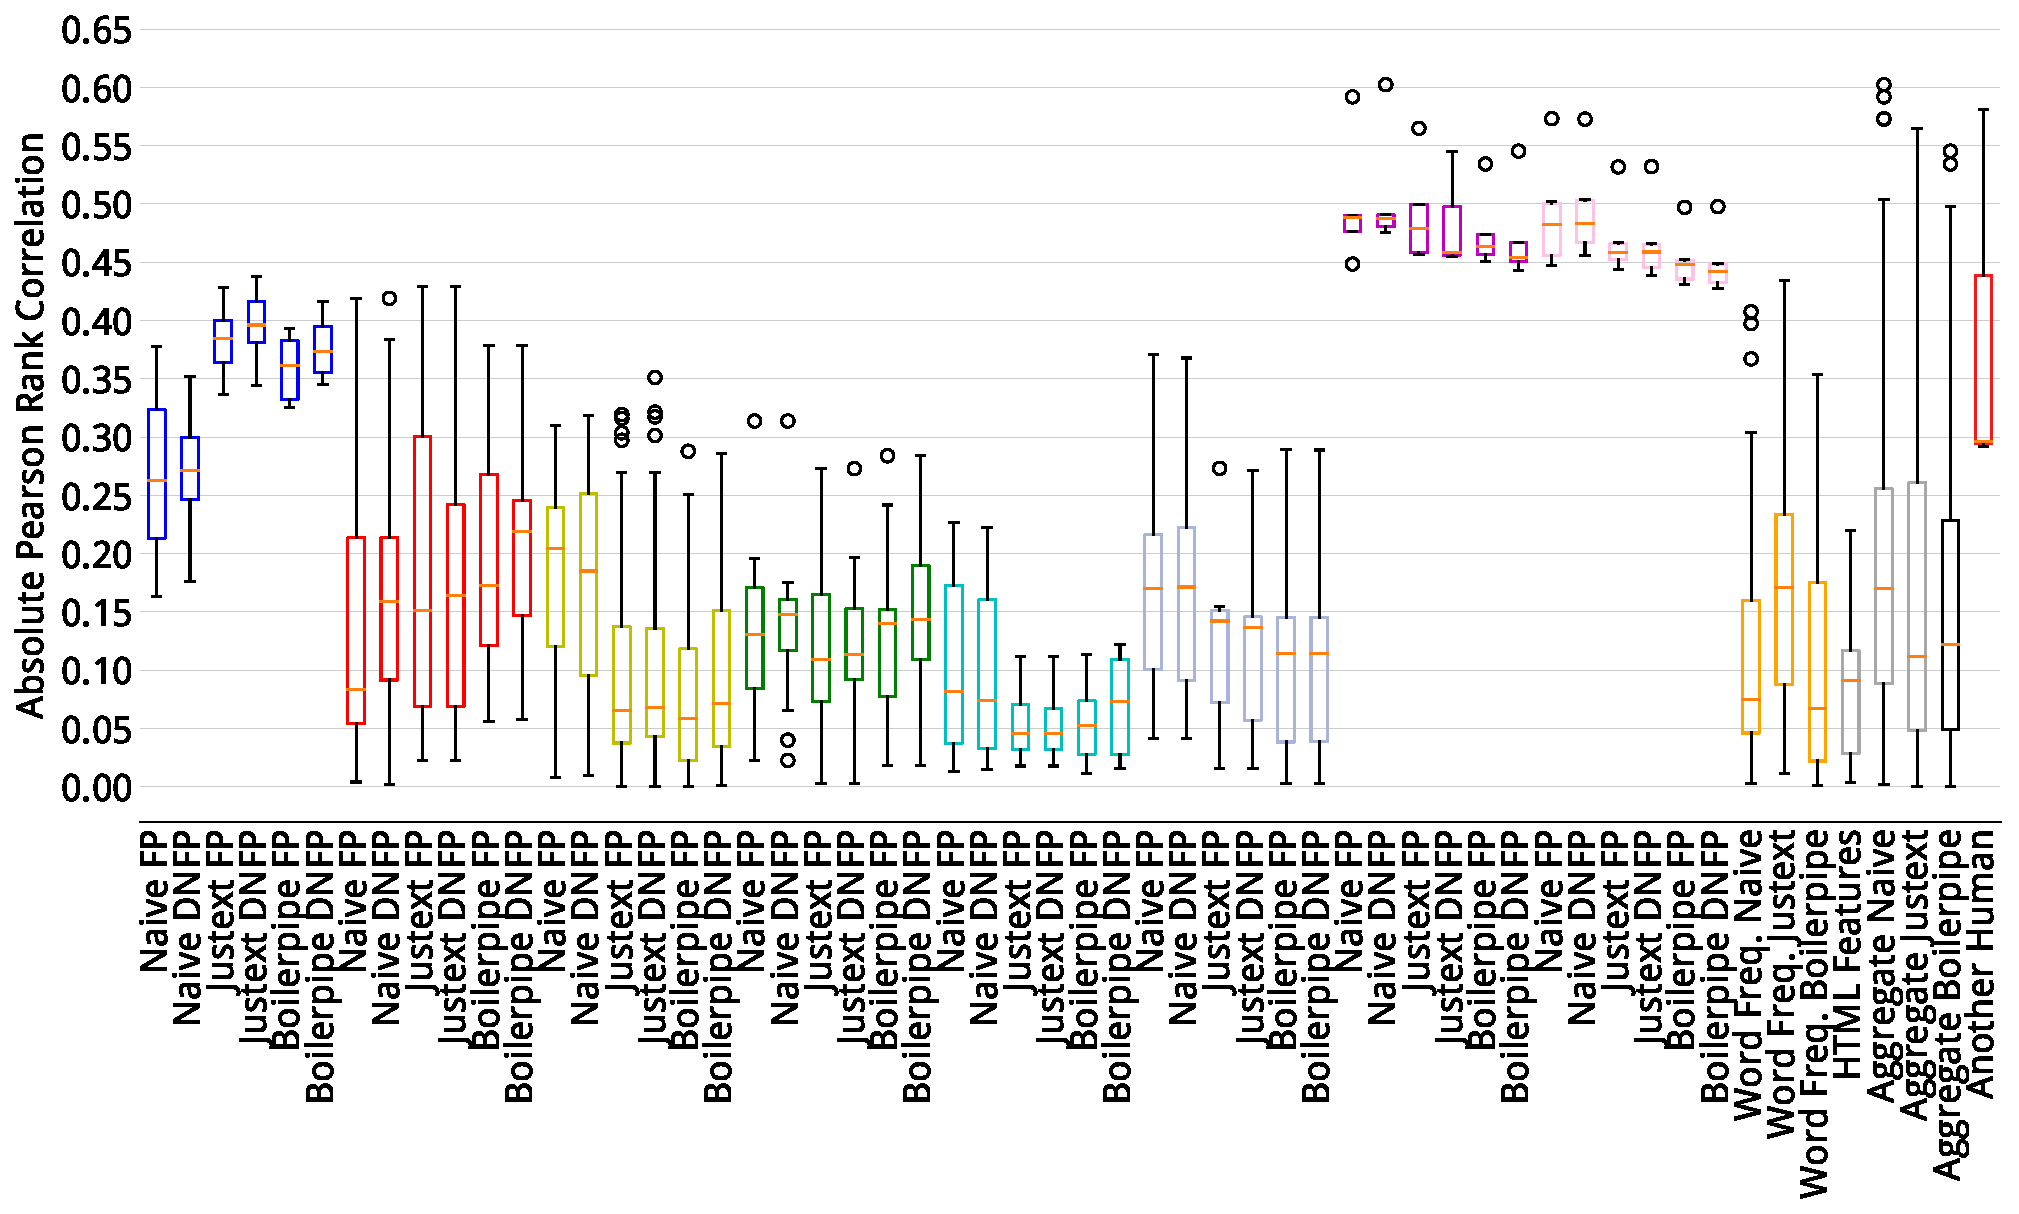
\includegraphics[width=0.70\textwidth]{graphics/box_pearson15_raw_values}
   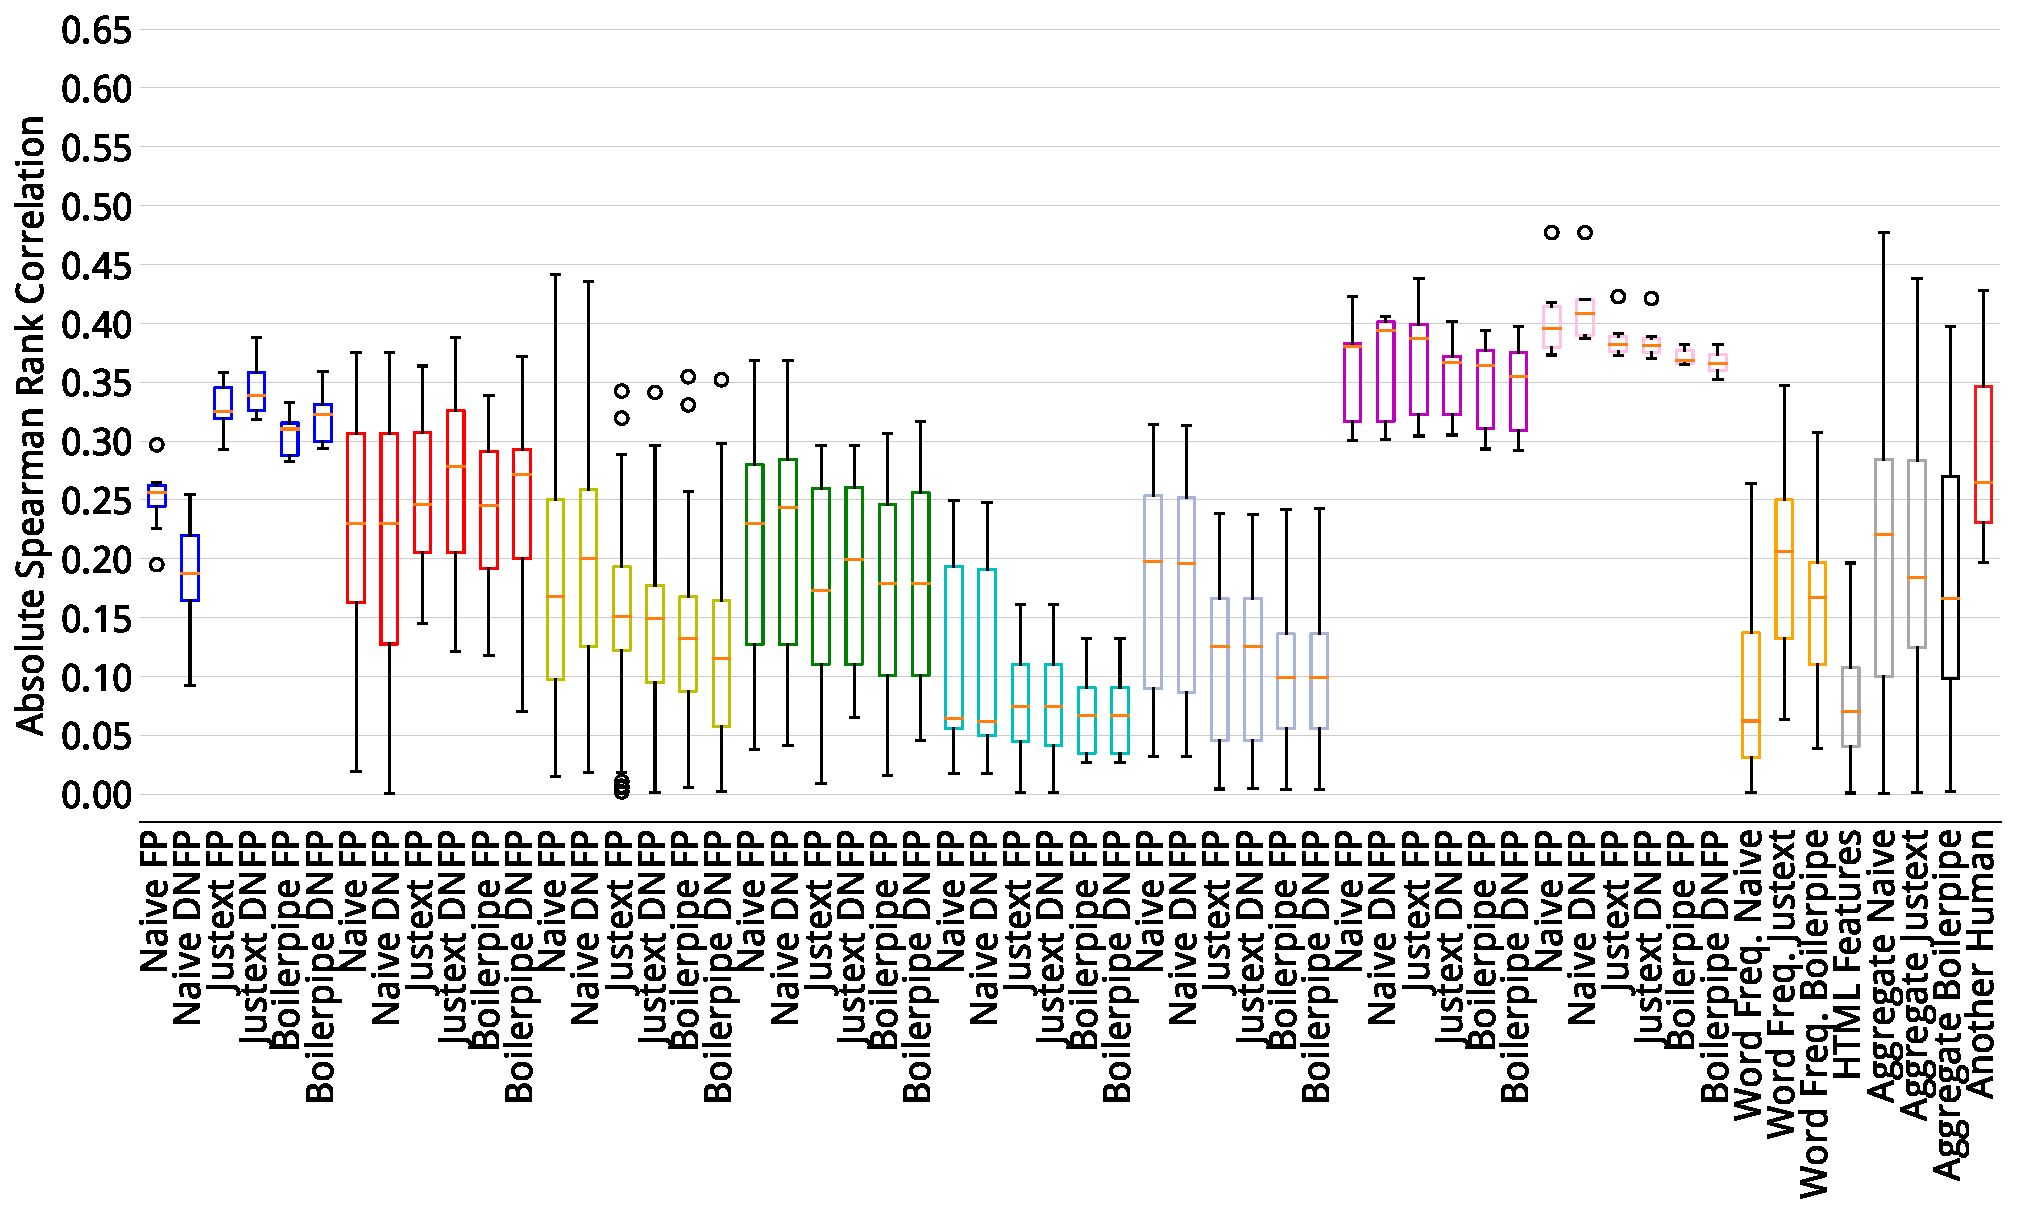
\includegraphics[width=0.70\textwidth]{graphics/box_spearman15_raw_values}
   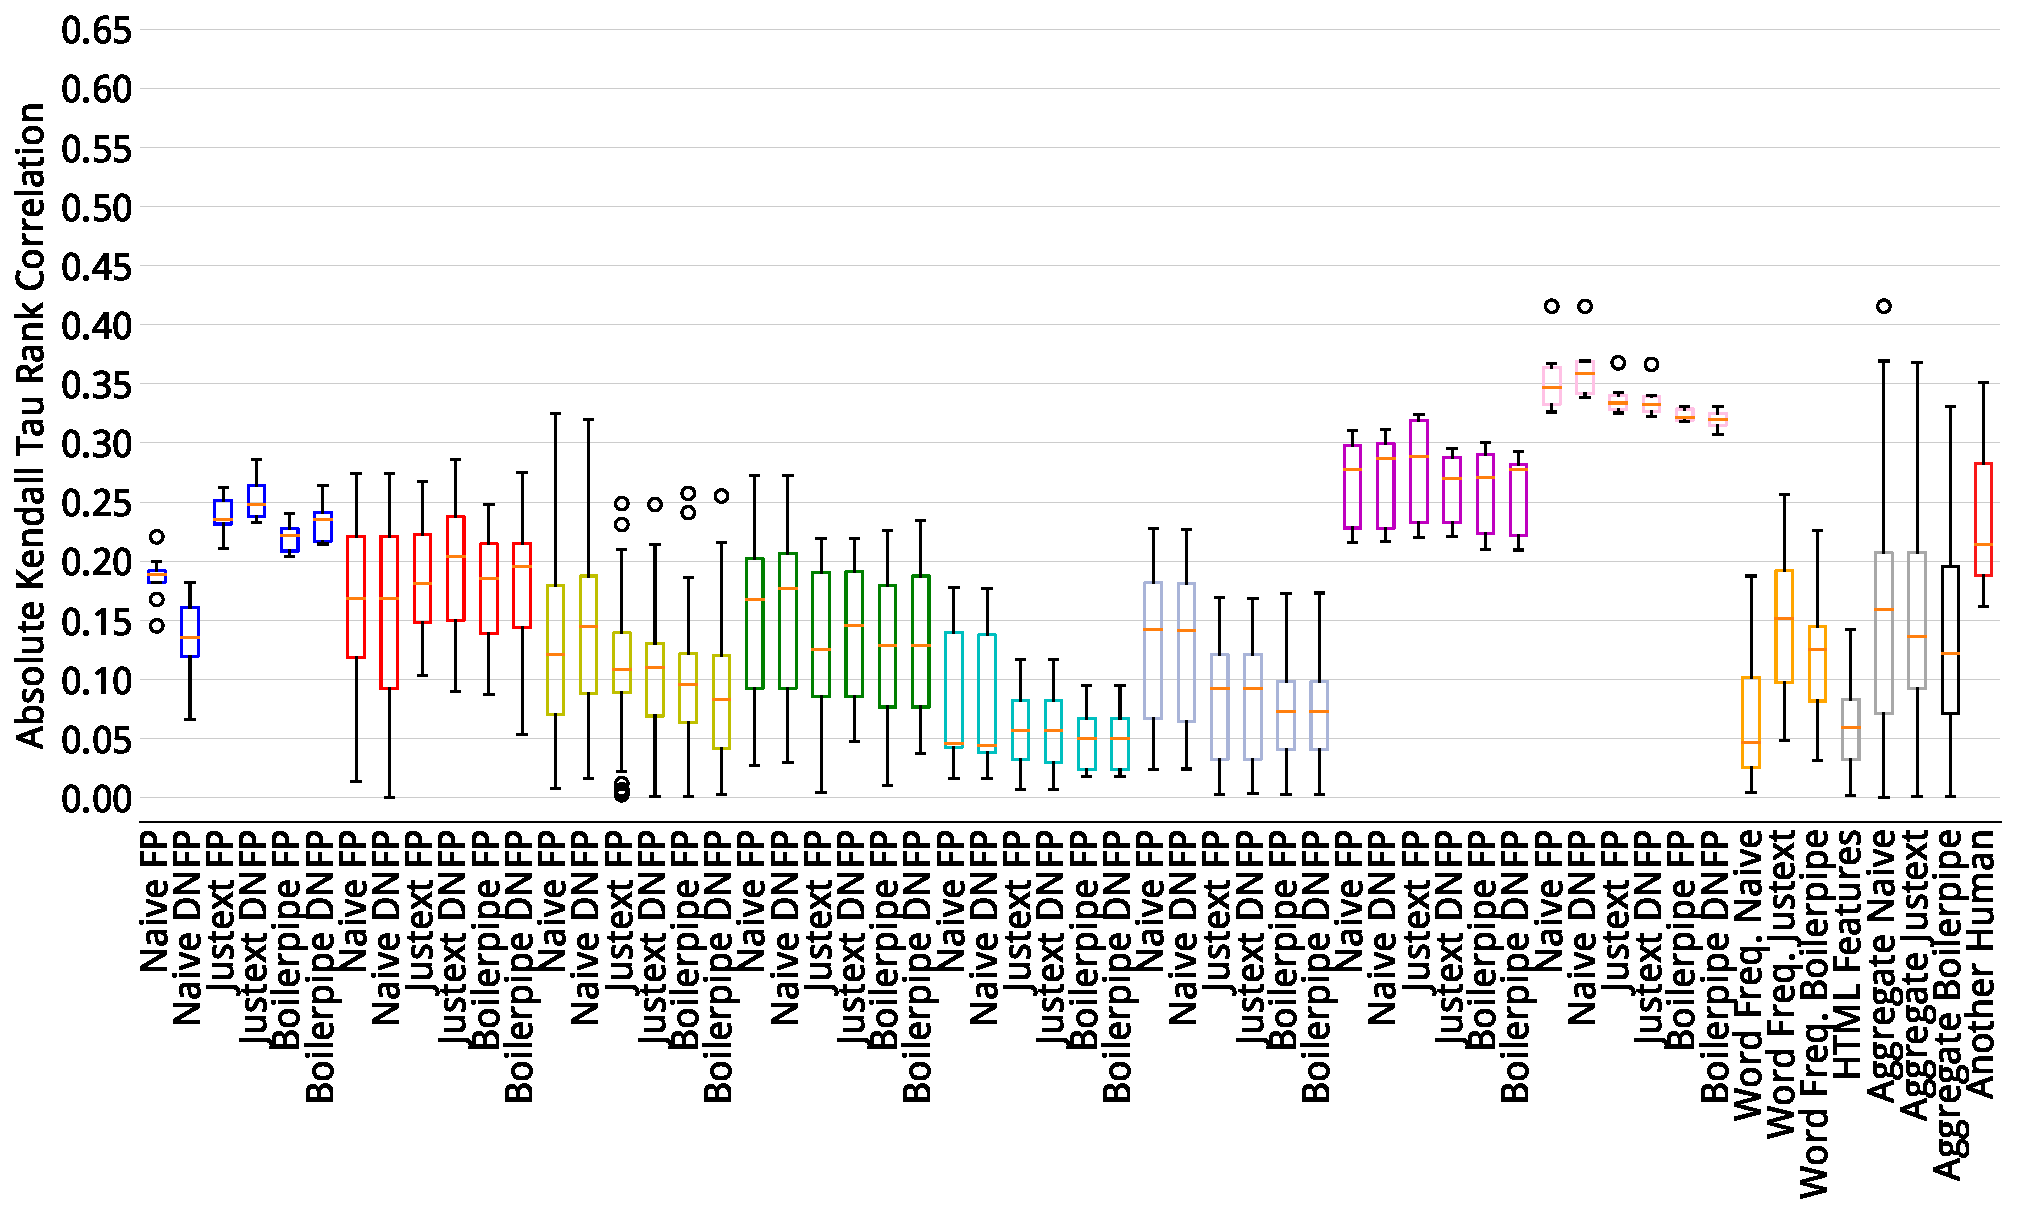
\includegraphics[width=0.70\textwidth]{graphics/box_kendalltau15_raw_values}
    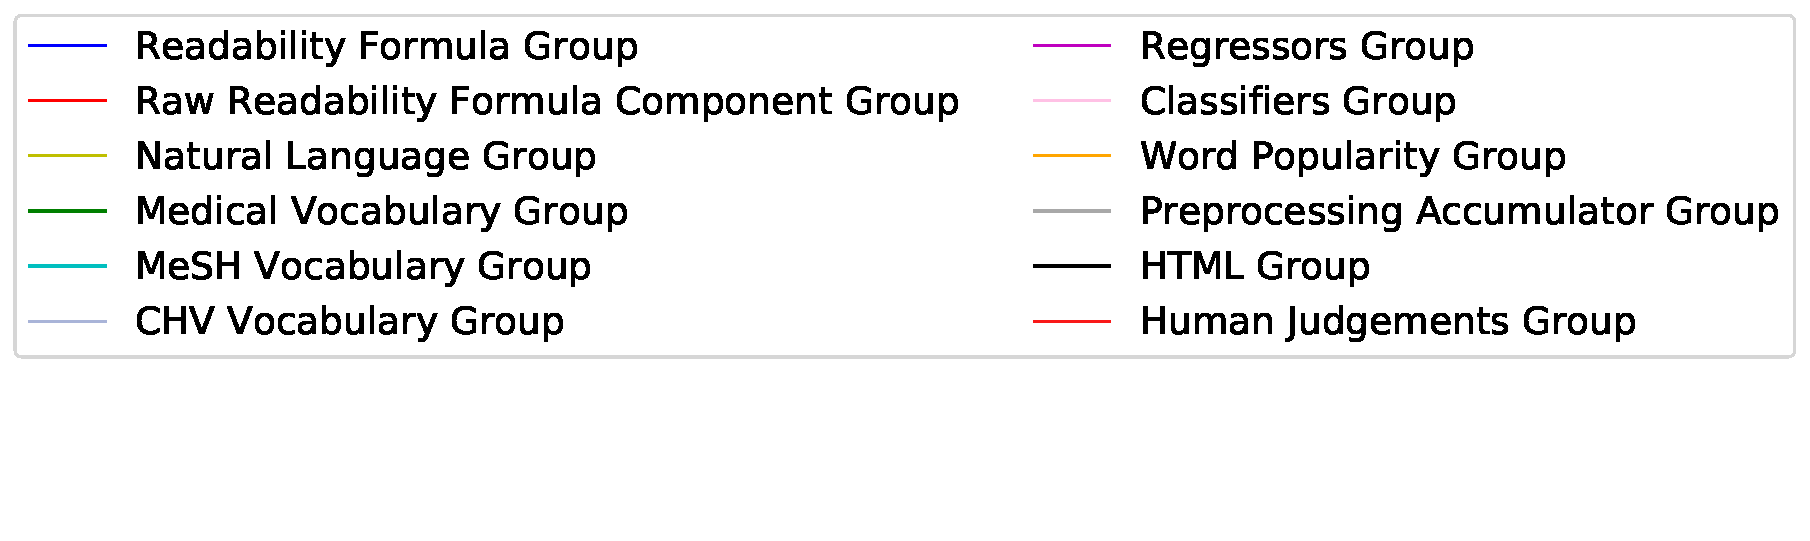
\includegraphics[width=0.65\textwidth]{graphics/legendCorr}
    \vspace{-1.cm}
    \caption{Box plots divided by feature groups. Correlations are calculated using understandability labels from relevant documents assessed in CLEF eHealth 2015}
   \label{fig:boxplot_corr_docs_2015}
\end{figure}

\begin{figure}[th!]
   \centering
   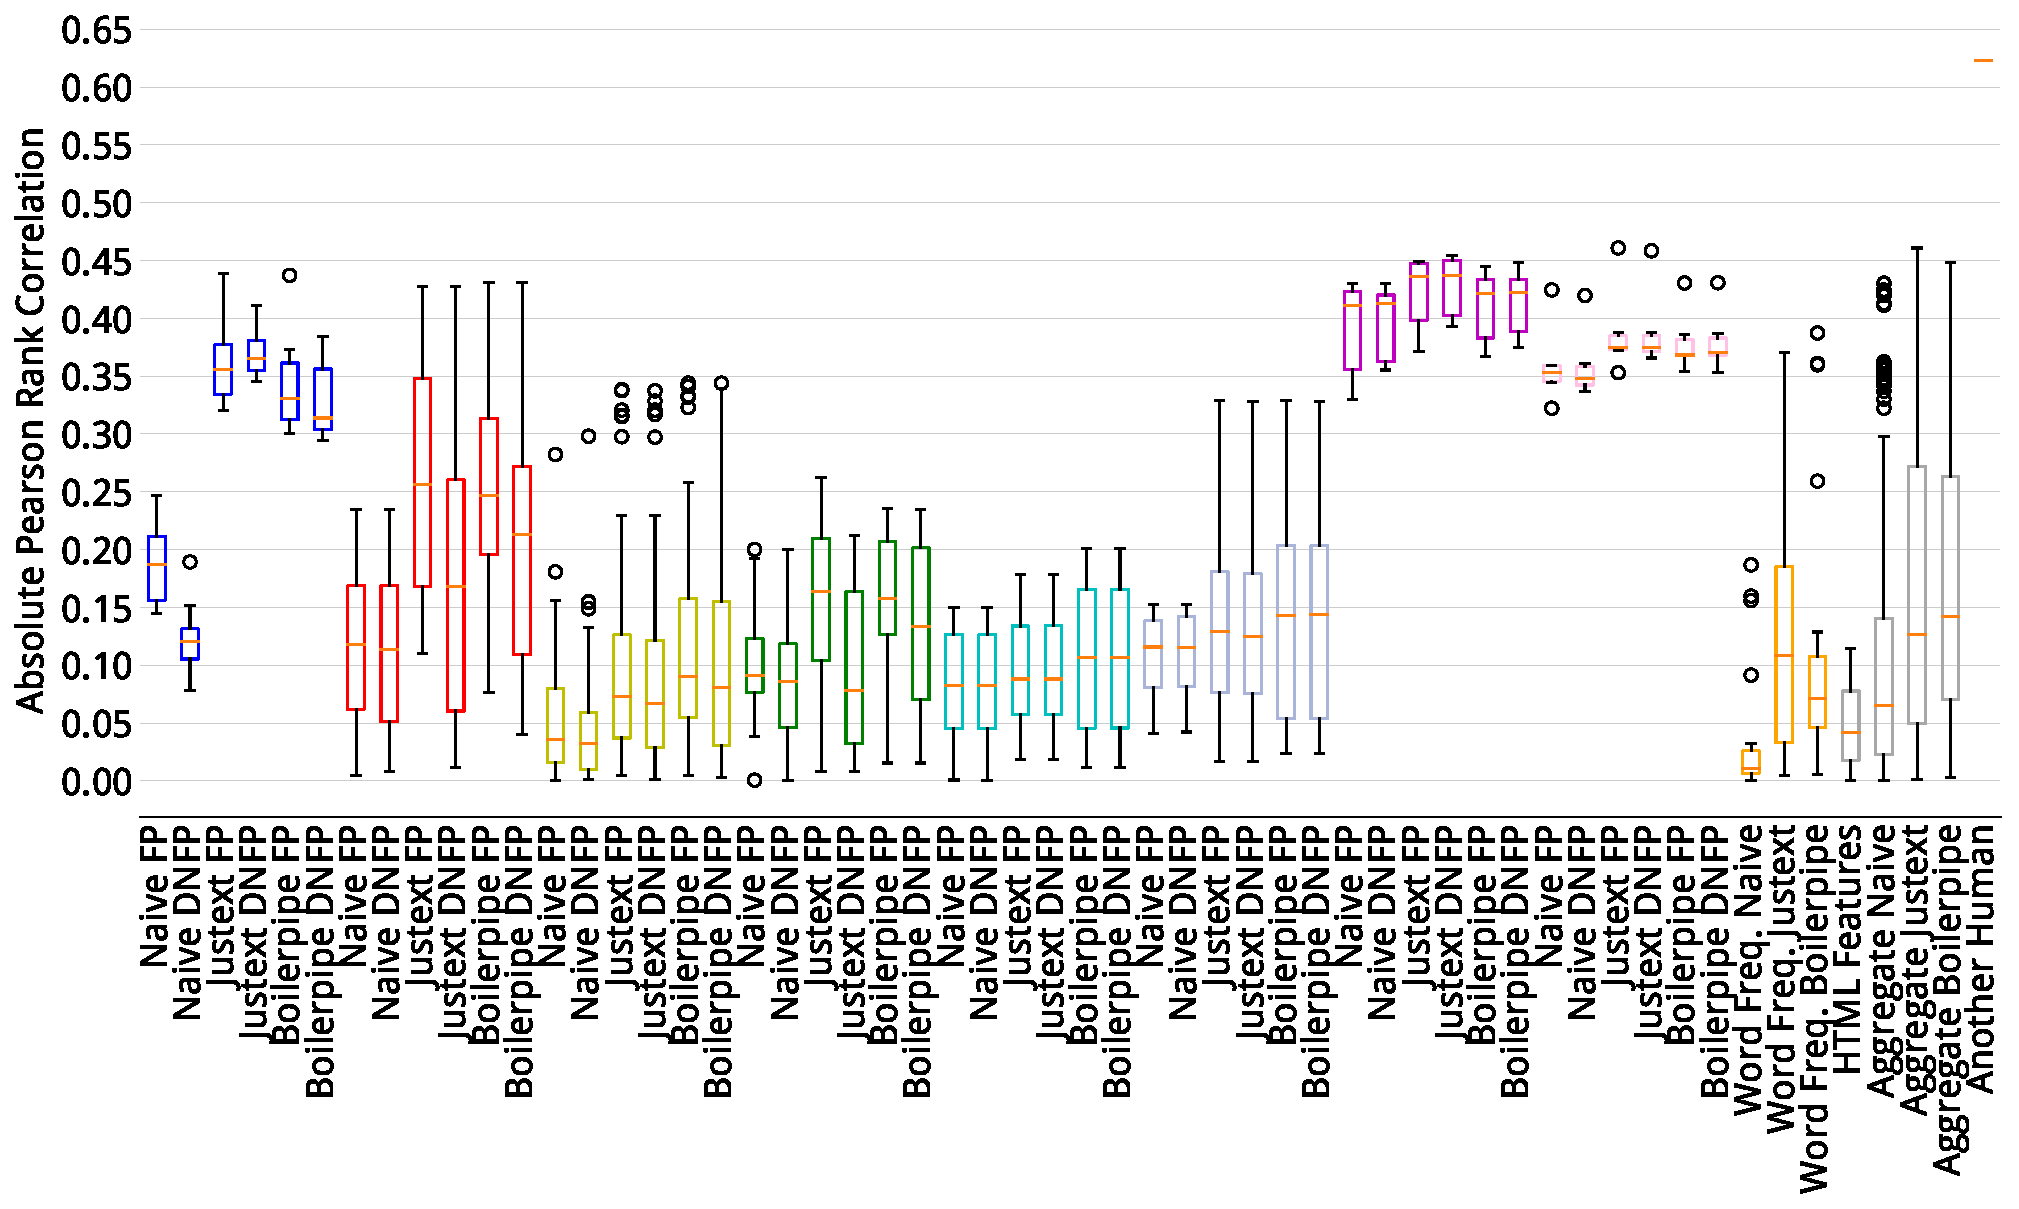
\includegraphics[width=0.70\textwidth]{graphics/box_pearson16_raw_values}
   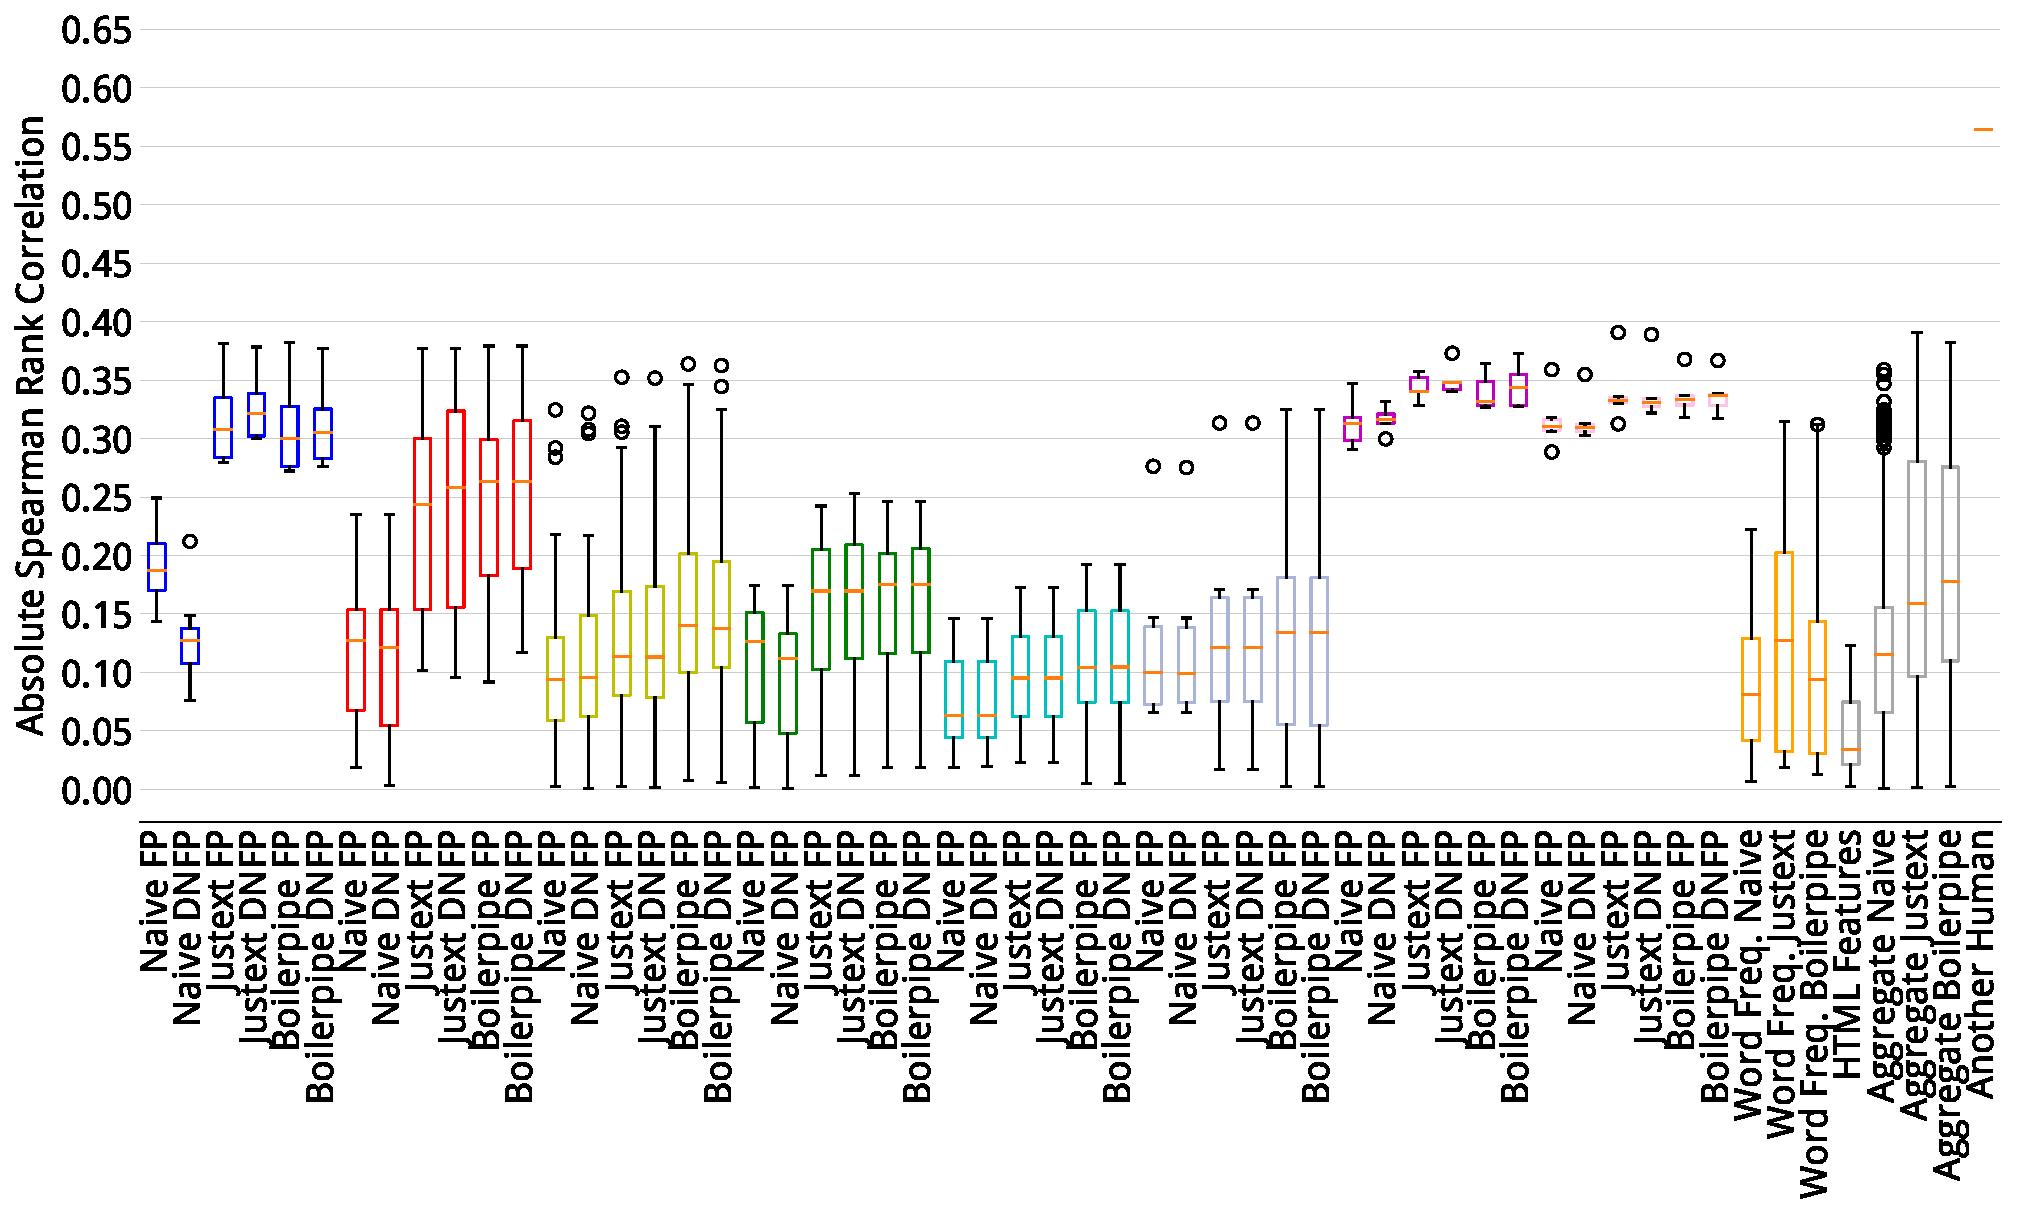
\includegraphics[width=0.70\textwidth]{graphics/box_spearman16_raw_values}
   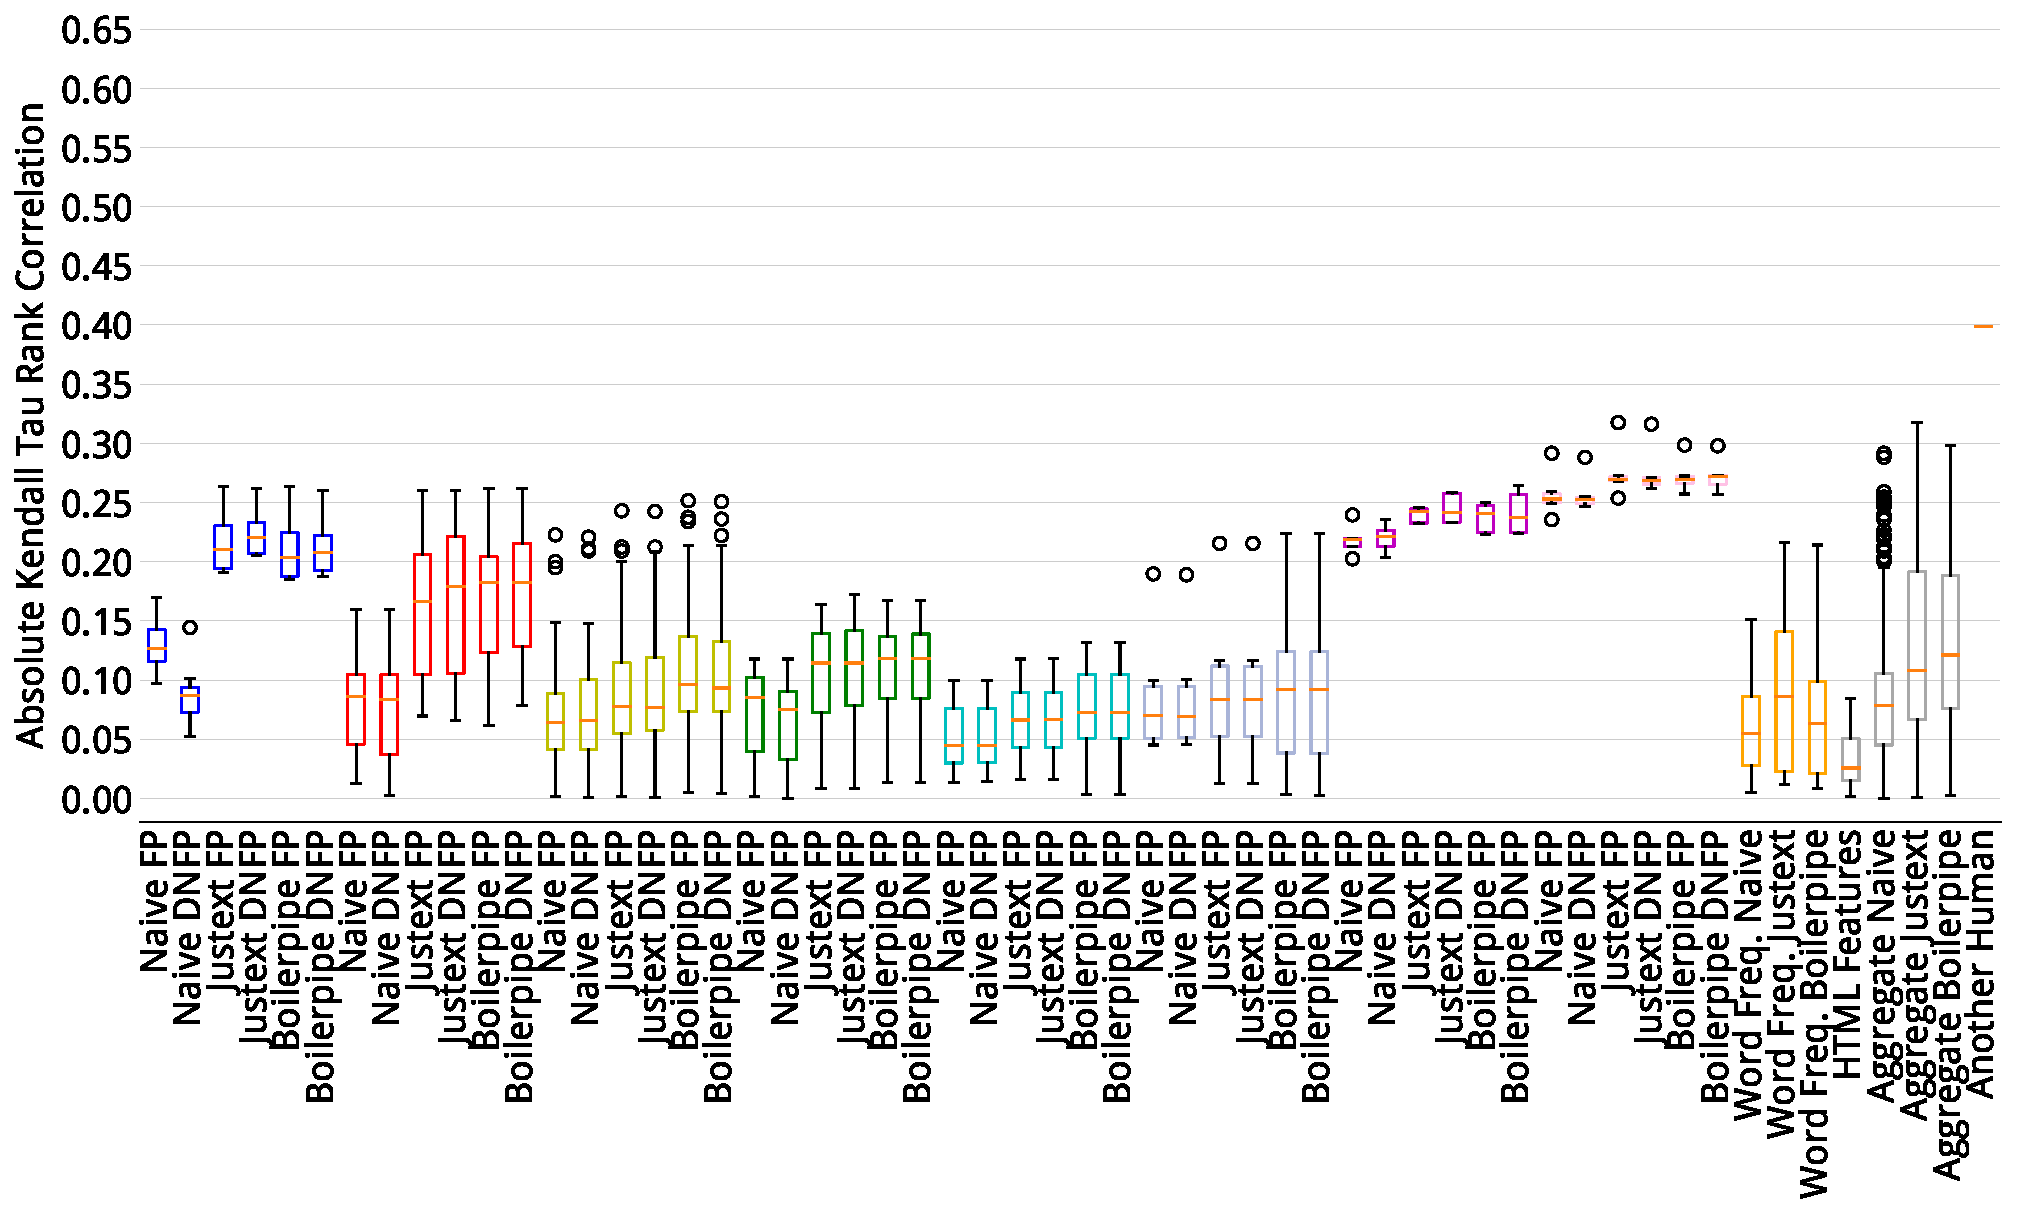
\includegraphics[width=0.70\textwidth]{graphics/box_kendalltau16_raw_values}
    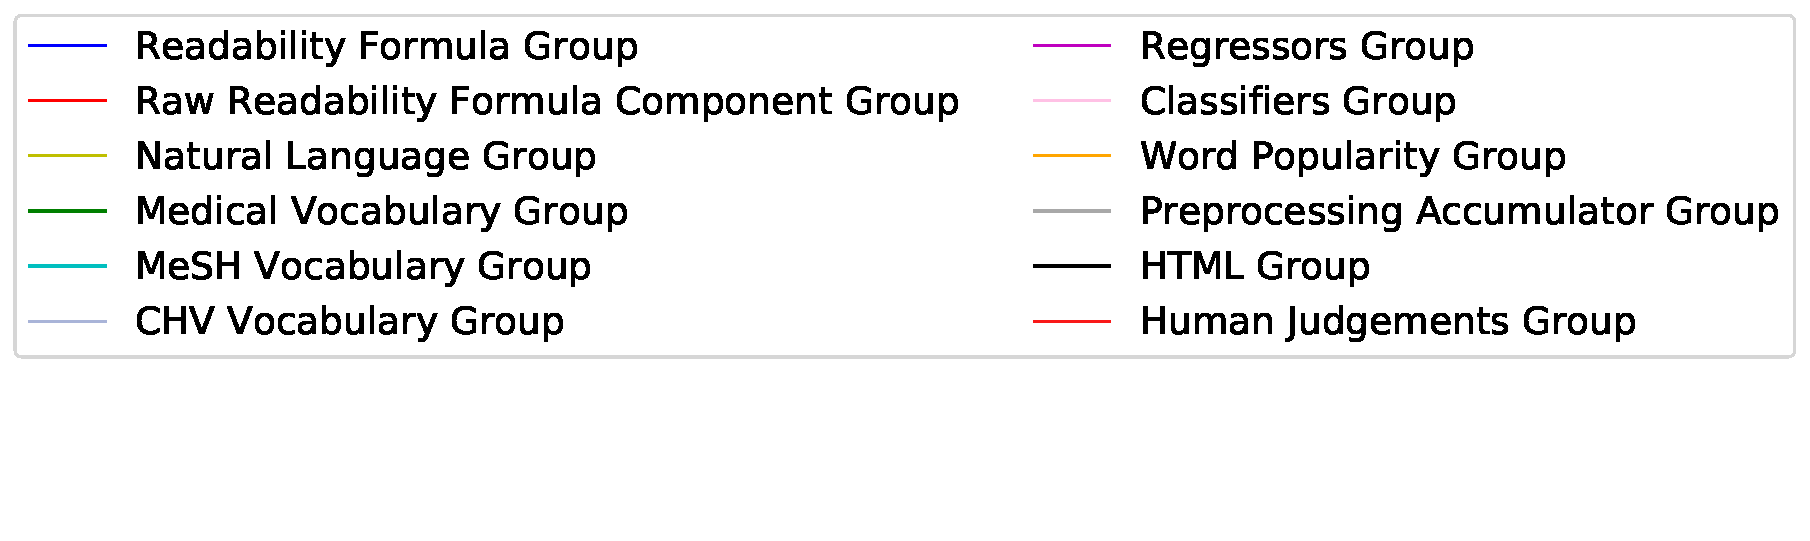
\includegraphics[width=0.65\textwidth]{graphics/legendCorr}
    \vspace{-1.cm}
    \caption{Box plots divided by feature groups. Correlations are calculated using understandability labels from relevant documents assessed in CLEF eHealth 2016}
   \label{fig:boxplot_corr_docs_2016}
\end{figure}

Figure~\ref{fig:boxplot_corr_docs_2015} shows the correlations for CLEF eHealth 2015 assessments.
The choice of preprocessing method had the highest impact on the traditional readability formula group, with the Naive preprocessing clearly underperforming the other preprocessing methods. The choice of the Naive method was also the worst with the raw readability formula components and word frequency estimators, but, interestingly, it was a good choice, if not the best one, for all other groups.
The highest correlations were archived by the regressors and classifiers, independently of the preprocessing method used.

%For this group, all correlation measures point out that the Naive processing yielded the weakest correlation, and Justext was marginally better than Boilerpipe. Comparing the medians, the strategy of DoNotForcePeriod performed better than ForcePeriod. The readability formula group was also the one with higher correlation, with an average correlation equal or higher than the human one.

Similarly to Figure~\ref{fig:boxplot_corr_docs_2015}, Figure~\ref{fig:boxplot_corr_docs_2016} reports the findings for CLEF eHealth 2016. This time, though, the Naive preprocessing method was clearly underperforming for most of the groups analysed, including regressors and classifiers.

In order to further understand our experiments, we compared the median of each pair of preprocessing strategy showed in Figures~\ref{fig:boxplot_corr_docs_2015} and~\ref{fig:boxplot_corr_docs_2016} and present the results in Table~\ref{tab:comparison_preprocessing}. 
For instance, the entry \textit{FP < DNFP} counts the number of times the median value for ForcePeriod was superior to DoNotForcePeriod when comparisons with the same HTML cleaning method was used, e.g. Naive ForcePeriod versus Naive DoNotForcePeriod. From all comparisons, the ones that were statistically significant according to a t-test are shown inside parentheses.

The upper part of Table~\ref{tab:comparison_preprocessing} shows results for the comparisons between ForcePeriod (FP) and DoNotForcePeriod (DNFP). Although the interpretation of readability formulas is drastically affected by this choice of preprocessing, as learning in Chapter~\ref{chp:preprocessing}, the correlation results are not.
The number of times FP reached a higher correlation than DNFP is roughly the same that DNFP was higher than FP.
The bottom part of Table~\ref{tab:comparison_preprocessing} shows the comparisons made for Naive, Justext and Boilerpipe. Results for CLEF 2015 contrast with 2016, while Naive was sightly better than Boilerpipe and Justext in 2015, it was the worst in almost all 2016 comparisons. Also, the comparisons between Justext and Boilerpipe are exactly the opposite from 2015 to 2016.

%
\begin{table}
\centering    
\caption{Exhaustive Comparison summary using the data from Figures 1.2 and 1.3. Numbers inside parentheses represent the number of tests that yielded p < 0.05 in a two-tailed t-test}
\label{tab:comparison_preprocessing}

\resizebox{1.\textwidth}{!}{
\begin{tabular}{lllllllll}
\toprule
\multirow{2}{*}{\textbf{Comparison}} & \multicolumn{4}{c}{\textbf{CLEF 2015}} & \multicolumn{4}{c}{\textbf{CLEF 2016}}\tabularnewline
\cmidrule(l{2pt}r{2pt}){2-5} \cmidrule(l{2pt}r{2pt}){6-9} 
& \textbf{Pearson} & \textbf{Spearman} & \textbf{Kendall Tau} & \textbf{Total} & \textbf{Pearson} & \textbf{Spearman} & \textbf{Kendall Tau} & \textbf{Total}\tabularnewline
\midrule
FP > DNFP & 8 (0) & 11 (4) & 11 (3) & 30 (7) & 16 (10) & 10 (3) & 11 (4) & 37 (17)\tabularnewline
FP < DNFP & 16 (5) & 12 (5) & 12 (6) & 40 (16) & 8 (0) & 12 (2) & 11 (2) & 31 (4)\tabularnewline
FP == DNFP & 0 & 1 & 1 & 2 & 0 & 2 & 2 & 4\tabularnewline
\midrule
Naive > Justext & 11 (7) & 9 (6) & 9 (5) & 29 (18) & 1 (0) & 0 (0) & 0 (0) & 1 (0)\tabularnewline
Naive < Justext & 6 (4) & 8 (4) & 8 (4) & 22 (12) & 16 (12) & 17 (13) & 17 (13) & 50 (38)\tabularnewline
Naive == Justext & 0 & 0 & 0 & 0 & 0 & 0 & 0 & 0\tabularnewline
Naive > Boilerpipe & 12 (7) & 10 (6) & 10 (5) & 32 (18) & 0 (0) & 0 (0) & 0 (0) & 0 (0)\tabularnewline
Naive < Boilerpipe & 5 (4) & 7 (3) & 7 (3) & 19 (10) & 16 (12) & 17 (13) & 17 (13) & 51 (39)\tabularnewline
Naive == Boilerpipe & 0 & 0 & 0 & 0 & 0 & 0 & 0 & 0\tabularnewline
Justext > Boilerpipe & 10 (7) & 16 (9) & 14 (8) & 40 (24) & 9 (4) & 9 (4) & 4 (2) & 17 (8)\tabularnewline
Justext < Boilerpipe & 7 (2) & 1 (0) & 3 (1) & 11 (3) & 8 (2) & 8 (2) & 13 (2) & 34 (6)\tabularnewline
Boilerpipe == Justext & 0 & 0 & 0 & 0 & 0 & 0 & 0 & 0\tabularnewline
\bottomrule 
\end{tabular}
} % close resizebox
\end{table}

%

%\section{Going Beyond Readability Measures}

%\begin{tabular}{lrlr}
%\toprule
%                                    Feature & Chi2 Value &  Features & MI Value \\
%\midrule
%     number\_chars\_nopreprocess &  3.99e+06 &                                   chv\_mean\_jst   &  0.1165 \\
%              number\_chars\_jst &  3.46e+06 &                      dale\_chall\_score\_jst\_fp   &  0.1090 \\
%              number\_chars\_bs4 &  2.90e+06 &              difficult\_words\_per\_word\_jst\_fp  &  0.1065 \\
% number\_syllables\_nopreprocess &  1.22e+06 &             difficult\_words\_per\_word\_jst\_nfp  &  0.1050 \\
%          number\_syllables\_jst &  1.11e+06 &                    coleman\_liau\_index\_jst\_fp   &  0.1030 \\
%          number\_syllables\_bs4 &  9.44e+05 &            number\_syllables\_per\_word\_jst\_nfp  &  0.0967 \\
%     number\_words\_nopreprocess &  7.24e+05 &             number\_syllables\_per\_word\_jst\_fp  &  0.0965 \\
%              number\_words\_jst &  6.07e+05 &                   longer\_10\_per\_word\_jst\_nfp  &  0.0957 \\
%       eng\_found\_nopreprocess &  5.50e+05 &                    longer\_10\_per\_word\_jst\_fp  &  0.0952 \\
%             number\_words\_bs4 &  5.21e+05 &                        chv\_mean\_nopreprocess     &  0.0931 \\
%                eng\_found\_jst &  4.68e+05 &                     dale\_chall\_score\_jst\_nfp   &  0.0930 \\
%  difficult\_words\_nopreprocess &  4.43e+05 &                    longer\_6\_per\_word\_jst\_nfp  &  0.0912 \\
%                 eng\_found\_bs4 &  3.96e+05 &                     longer\_6\_per\_word\_jst\_fp  &  0.0903 \\
%           difficult\_words\_jst &  3.67e+05 &                   flesch\_reading\_ease\_jst\_fp   &  0.0901 \\
%         longer\_4\_nopreprocess &  3.38e+05 &                  flesch\_reading\_ease\_jst\_nfp   &  0.0895 \\
%                  longer\_4\_jst &  3.33e+05 &               longer\_10\_per\_sentence\_jst\_nfp  &  0.0854 \\
%           difficult\_words\_bs4 &  3.30e+05 &                   coleman\_liau\_index\_jst\_nfp   &  0.0839 \\
%  stopwords\_found\_nopreprocess &  2.98e+05 &                            lix\_index\_jst\_nfp    &  0.0837 \\
%                n\_chv\_concepts &  2.82e+05 &         difficult\_words\_per\_sentence\_jst\_nfp  &  0.0822 \\
%                  longer\_4\_bs4 &  2.75e+05 &   number\_polysyllable\_words\_per\_word\_jst\_nfp &  0.0815 \\ 
%\bottomrule
%\end{tabular}

%\begin{tabular}{|c|c|c|c|c|c|c|c|c|c|}
%\hline 
%\multirow{2}{*}{Feature Group} & \multicolumn{3}{c|}{Chi} & \multicolumn{3}{c|}{Multual Information} & \multicolumn{3}{c|}{Goodman Kruskal}\tabularnewline
%\cline{2-10} 
% & Top 10 & Top 20 & Top50 & Top 10 & Top 20 & Top 50 & Top 10 & Top 20 & Top 50\tabularnewline
%\hline 
%Justext &  &  & 6 &  &  &  &  &  & \tabularnewline
%\hline 
%BS4 &  &  & 6 &  &  &  &  &  & \tabularnewline
%\hline 
%No Preprocessing &  &  & 7 &  &  &  &  &  & \tabularnewline
%\hline 
%Force Period &  &  & 0 &  &  &  &  &  & \tabularnewline
%\hline 
%Do Not Force Period &  &  & 0 &  &  &  &  &  & \tabularnewline
%\hline 
%HTML Features &  &  &  &  &  &  &  &  & \tabularnewline
%\hline 
%Readability Features &  &  &  &  &  &  &  &  & \tabularnewline
%\hline 
% &  &  &  &  &  &  &  &  & \tabularnewline
%\hline 
%\end{tabular}
%

%\section{Discussion}
%\label{sec:discussion}


\section{Summary}
\label{sec:conclusion_doc_analysis}

There is an abundance of factors that affect how readability is perceived by users. 
In this chapter we devised and studied a large number of readability estimators, ranging from traditional readability formulas extensively used in the past 50 years to state-of-the-art machine learning algorithms.
We grouped them into semantically related groups in order to visualize their correlation with human assessments collected during CLEF eHealth campaigns in 2015 and 2016.

Complementary to our previous chapter, we evaluated how preprocessing steps impact the readability estimation in traditional readability formulas and in other modern estimators. We empirically learnt the importance of preprocessing steps when applying readability formulas, as the highest correlations happen when other than the Naive method is used.
For the most modern estimators, such as the ones based on machine learning methods, the correlation is less sensible to the preprocessing steps.

We also studied the correlation of each individual readability formula to the human assessment to provide insights on which formula should be preferred. Our analysis concluded that the Simple Measure of Gobbledygook (SMOG) and Dale-Chall Index (DCI) were the most correlated metrics for the two datasets studied and, together with Coleman-Liau Index (CLI) and the Flesch Reading Ease (FRE) are the most stable metrics across datasets, and therefore, should be preferred.

Finally, this chapter serves as a basis for the following chapters of this work, as the learning to rank methods will largely use the estimators devised and analysed here.

%MISSING - POSSIBLE TODOs:
% * I will use the evaluations from CLEF eHealth 2015 and 2016 to conclude that for the same topic, we can find very different results in respect to their understandability (readability) score. I might want to hire some people to classify how hard a topic is. Then I could correlate that with the mean scores of documents for that topic.
% * I will try to come up with some sort of reasoning behind the understandability judgements: is it because of the text length? number of hard (long or out of dictionary) words?

%\mytodo{In this chapter I could add other readability measures later, such as the neural network ones (see cikm 2017)}





\bibliographystyle{abbrv}
\bibliography{main}

\end{document}
